\documentclass[12pt]{article}

\usepackage[utf8]{inputenc}
%\usepackage[T1]{fontenc}

\usepackage{geometry}
\geometry{a4paper}
\geometry{left=2.5cm,right=2.5cm,top=2.5cm,bottom=2.5cm}
\usepackage{graphicx}
\graphicspath{{./images/}}

\usepackage{float}
\usepackage[italian]{babel}
\usepackage{hyperref}
\usepackage{wrapfig}
\usepackage{amsmath}
\usepackage{listings}

\usepackage{color}

\definecolor{pblue}{rgb}{0.13,0.13,1}
\definecolor{pgreen}{rgb}{0,0.5,0}
\definecolor{pred}{rgb}{0.9,0,0}
\definecolor{pgrey}{rgb}{0.46,0.45,0.48}

\usepackage{listings}
\lstset{language=Java,
  showspaces=false,
  showtabs=false,
  breaklines=true,
  numbers=left,
  xleftmargin=4.5ex,
  basicstyle=\ttfamily\footnotesize,
  showstringspaces=false,
  breakatwhitespace=true,
  commentstyle=\color{pgreen},
  keywordstyle=\color{pblue},
  stringstyle=\color{pred},
  moredelim=[il][\textcolor{pgrey}]{$$},
  moredelim=[is][\textcolor{pgrey}]{\%\%}{\%\%}
}

\linespread{1.2}
\setlength{\parindent}{0pt}

\begin{document}

%----------------------------------------------------------------------------------------
%	TITOLO
%----------------------------------------------------------------------------------------

\begin{titlepage}

\newcommand{\HRule}{\rule{\linewidth}{0.5mm}}

\center

\textsc{\Large Relazione di progetto di "Smart City e Tecnologie Mobili"}\\[0.5cm]

\begin{figure}[H]
  
\includegraphics[width=0.5\textwidth]{logo.png}
  \centering
\end{figure}

\HRule \\[0.5cm]
{ \large Incentivo alla sostenibilità nel settore ospitality tramite gamification}\\[0.4cm]
\HRule \\[1.5cm]

\vfill

\begin{flushleft}
\emph{Numero del gruppo: 3}\\[1cm]
\emph{Componenti del gruppo: Alan Mancini, Alberto Marfoglia, Matteo Brocca}\\[3cm]
\end{flushleft}



\end{titlepage}

%----------------------------------------------------------------------------------------
%	INDICE
%----------------------------------------------------------------------------------------

\tableofcontents

\newpage

%----------------------------------------------------------------------------------------
%	INTRODUZIONE
%----------------------------------------------------------------------------------------

\section{Introduzione}

La sostenibilità in Europa è un tema molto sentito anche nel settore alberghiero, da anni infatti sono presenti sistemi e centraline che permettono di ridurre gli sprechi energetici andando ad esempio a spegnere gli impianti elettrici all'uscita dell'ospite dalla sua camera.

Negli USA invece la maggior parte degli hotel non dispone di questi semplici meccanismi e l'utenza è molto meno attenta al problema eco sostenibilità. Un banale esempio di spreco energetico che si presenta con un'elevata frequenza, è quello in cui l'ospite, specialmente d'estate, esce dalla camera lasciando il condizionatore acceso a temperature molto basse e contemporaneamente le tende aperte.

Dal 2020 la \href{https://sustainablehospitalityalliance.org/}{Sustainable Hospitality Alliance}, che comprende il 30\% dell'industria alberghiera globale, si impegna a proporre linee guida e \textit{best practice} per il design e la gestione di hotel sostenibili. Tuttavia il processo per la sostenibilità è molto lungo ed impegnativo e l'alleanza è ancora in una fase preliminare di raccolta dati.

Inoltre il World Tourism Organization ha divulgato un documento che riassume alcuni atteggiamenti utili a ridurre i consumi prodotti dal turismo. Secondo un rapporto della Commissione Europea (‘Consumption and Environment’), il settore economico del turismo si colloca al quarto posto pre fabbisogno energetico. Infine uno studio della Confesercenti rilasciato ad agosto 2022, prevede un aumento delle bollette per gli hotel di oltre 1.5 miliardi di euro nei prossimi 12 mesi.

Il nostro obiettivo è quello di proporre all'alleanza sopracitata Ecotrip, un nuovo sistema che faccia leva direttamente sugli ospiti promuovendone un comportamento virtuoso in termini di consumi energetici/idrici. 

Il sistema è composto da una centralina, da installare nella camera d'albergo, che attraverso diversi sensori rileva i consumi di energia ed acqua e li carica su infrastruttura cloud.
In particolare la centralina misura i consumi di energia elettrica relativi al circuito luci e al circuito prese, il flusso di acqua fredda e calda con relative temperature,
la temperatura e umidità d'ambiente ed infine è in grado di determinare se le tende sono aperte o chiuse con sensori di luminosità ambientale.

Gli ospiti attraverso un'apposita applicazione su smartphone ottengono un "punteggio sostenibilità" calcolato in base al comportamento tenuto durante il proprio periodo di pernottamento, il punteggio 
può essere convertito in uno sconto al checkout. Per accedere ai dati del proprio pernottamento, all'ospite è richiesto semplicemente di avvicinare il suo smartphone ad un tag NFC installato all'interno della sua stanza.
Il tag è collegato e gestito dalla centralina che lo riprogramma per ogni pernottamento inserendovi il relativo token di accesso, garantendo così la privacy degli ospiti che saranno in grado di accedere solo ai propri dati.

Infine, il gestore dell'albergo dispone di un pannello di controllo per monitorare i dati delle varie stanze e gestire i pernottamenti.

Il sistema Ecotrip è pensato per essere installato in aggiunta alle centraline ed impianti già esistenti nelle stanze degli Hotel. 
Con Ecotrip l'ospite viene direttamente sensibilizzato alla eco-sostenibilità grazie a concetti di "gamification".

%Il contributo tecnologico apportato dal progetto si riassume in una centralina (\textit{control unit}) installa in ogni stanza, una piattaforma in \textit{cloud} per la raccolta dei dati e un' applicazione lato smartphone che permette di mostrare all'ospite un "punteggio sostenibilità" che ne evidenza l'attitudine al corretto consumo delle risorse o viceversa allo spreco. La centralina consiste in un computer/micro-controllore che esegue un servizio sviluppato ad-hoc, il quale interroga periodicamente sensori dislocati nella stanza. Questi rilevano fattori ambientali come illuminazione e temperatura della stanza ma anche consumi elettrici/idrici.

Il contributo tecnologico apportato dal progetto comprende:
\begin{itemize}
    \item l'ingegnerizzazione della centralina che si occupa di rilevare periodicamente fattori ambientali e consumi elettrici/idrici tramite sensori opportunamente connessi e programmati; questa si occupa anche di inviare i dati campionati sulla piattaforma cloud e di gestire il tag NFC. 
    \item Impiego della piattaforma cloud Amazon AWS per realizzare un'infrastuttura a microservizi che permetta la gestione delle centraline (AWS IoT Core), memorizzare i dati (AWS DynamoDB), gestire gli account/autenticazioni (AWS Cognito), calcolare i punteggi sostenibilità e generare le autorizzazioni per i visitatori con funzioni \textit{lambda}, ed infine fornire il pannello di controllo e l'app (AWS EC2 / S3).
    \item Sviluppo applicativo composto da frontend (React) e backend (Nodejs) utilizzata sia dagli amministratori di Ecotrip, sia dagli albergatori. 
    \item Sviluppo web app (React) che consente all'ospite di visualizzare il proprio "punteggio sostenibilità" associato ad un determinato pernottamento.
\end{itemize}


\newpage 
%----------------------------------------------------------------------------------------
%	STATO DELL'ARTE
%----------------------------------------------------------------------------------------

\section{Stato dell'arte}

Riassumere le soluzioni presenti in letteratura inerenti al problema in esame. Per ciascuna, discutere le principali diversità o affinità rispetto al progetto presentato. Nel caso non siano presenti soluzioni direttamente comparabili a quella presentata descrivere comunque le principali tecniche note per affrontare la tematica trattata.\\

Le soluzioni esposte devono essere corredate degli opportuni riferimenti bibliografici. Nel caso si tratti di soluzioni già operative sul mercato, devono essere indicate le fonti (online) dove poter accedere al servizio o approfondirne i contenuti.\\


Vincoli circa la lunghezza della sezione (escluse didascalie, tabelle, testo nelle immagini, schemi):

\vspace{1cm}
\begin{tabular}{l|rr}
 & Numero minimo di battute & Numero massimo di battute \\
 \hline
 1 componente & 2000 & 3000 \\
 2 componenti & 2500 & 4500 \\
 3 componenti & 3000 & 6000 \\
 \hline
\end{tabular}


\newpage

%----------------------------------------------------------------------------------------
%	ANALISI DEI REQUISITI
%----------------------------------------------------------------------------------------

\section{Analisi dei requisiti}

%In questa sezione esporre brevemente i requisiti a cui il sistema proposto deve rispondere, concentrando l'attenzione sugli aspetti più rilevanti e facendo eventualmente uso di opportuni diagrammi di alto livello.\\

%  3 componenti & 8000 & 10000 \\

Riportiamo prima in prosa i requisiti utente completi, derivanti da alcune sessioni di 
knowledge crunching con il nostro partner che rappresenta l'esperto di dominio.
Successivamente riportiamo un analisi tecnica preliminare del sistema con
i requisti di sistema a punti. 

\subsection{Requisiti utente}

Il gestore di un hotel, l'albergatore, può supportare il sistema Ecotrip
installando la centralina in una o più camere. Una centralina comprende diversi
sensori cablati che andranno opportunamente sistemati all'interno della camera.
I sensori previsti per il primo prototipo di Ecotrip sono:

\begin{itemize}
    \item 1 sensore per rilevare il consumo elettrico
    \item 1 flussometro per misurare il consumo d'acqua fredda + 1 per l'acqua calda
    \item 1 termometro per misurare la temperatura dell'acqua fredda + 1 per l'acqua calda
    \item 1 sensore di luminosità per ogni finestra, per rilevare se la tenda è aperta o chiusa
    \item 1 sensore di temperatura ambientale
    \item 1 sensore di umidità ambientale
\end{itemize}

La centralina comprende anche un insieme di sensori per identificare se l'ospite
è presente nella camera o meno: questo specifico aspetto viene lasciato per
sviluppi successivi al primo prototipo, il quale "rileverà" la presenza
dell'ospite attraverso un semplice interruttore meccanico. Nel prodotto finale
prevediamo invece due possibilità:
\begin{itemize}
    \item nel caso in cui la camera dispone già di una centralina che accende e spegne
    l'impianto elettrico in base all'inserimento della chiave da parte
    dell'ospite, allora la nostra centralina identificherà la presenza in base
    all'attivazione degli impianti.
    \item negli altri casi doteremo la camera di un sensore per identificare se la porta
    di accesso è aperta/chiusa e di uno o più sensori di presenza da installare a
    soffitto, in modo da stabilire se l'ospite è entrato o uscito ogni volta che
    la porta viene chiusa.
\end{itemize}

Una volta installata, la centralina viene connessa alla rete wifi dell'hotel in
modo da consentirle l'accesso ad Internet, inoltre viene configurata abbinandola
al numero di camera. Dopo la configurazione, la centralina campionerà ogni X
secondi i dati da tutti i sensori e li invierà sul cloud: deve essere possibile
stabilire l'origine dei dati nei termini di hotel e camera. Infine il sistema
deve prevedere meccanismi di controllo dello stato (centralina online/offline) e
di manutenzione da remoto.

Gli amministratori di Ecotrip tramite un pannello di controllo web possono
gestire la lista degli hotel, le loro camere, visualizzare lo stato delle
centraline installate ed infine registrare l'account dell'albergatore.

L'albergatore potrà quindi accedere al pannello di controllo e, per ciascuna
delle sue camere, visualizzare i dati istantanei raccolti dai sensori ed
indicare i momenti di check-in e check-out di un ospite: quest'ultima funzione
manuale, in ottica di sviluppo futuro, sarà automatizzabile con la connessione
del pannello di controllo al gestionale dell'albergo.

Per ogni soggiorno, cioè il periodo tra il check-in ed il check-out dell'ospite,
saranno visualizzabili oltre che i dati sintetizzati, anche il consumo totale di
CO2 ed il punteggio "sostenibilità" ottenuto. Il calcolo della CO2 viene fatto
considerando il consumo elettrico utilizzato per alimentare la stanza, compreso
quello per il suo riscaldamentoe e quello stimato per riscaldare l'acqua: si
considera infatti che negli USA le camere vengono riscaldate unicamente con
pompa di calore e non si utilizza gas/metano. Per effettuare il calcolo CO2 deve
essere specificato per ciascun hotel il costo dell'energia nei termini di
CO2/Kilowatt. Il punteggio "sostenibilità" tiene conto, non solo della CO2
totale, ma anche del comportamento tenuto dall'ospite durante la sua permanenza.
Alcuni comportamenti penalizzanti sono:

\begin{itemize}
    \item il fatto di uscire dalla camera lasciando in periodo estivo di giorno tende aperte e condizionatore acceso a pieno regime.
    \item usare eccessiva acqua
\end{itemize}

L'ospite attraverso l'app Ecotrip può visualizzare i dati del suo soggiorno
corrente e di quelli passati, comprendenti sia i dati sintetizzati, che il
consumo CO2 ed il punteggio "sostenibilità" aggiornati in tempo reale.

Al fine di permettere all'ospite di collegarsi facilmente ed autonomamente ai
dati del proprio soggiorno, a quest'ultimo viene associato un token univoco,
contenente un codice casuale generato al momento del check-in, ed inviato alla
centralina della relativa camera. Alla centralina è collegato un transponder NFC
che deve essere installato nella camera in modo che sia visibile agli ospiti,
magari identificabile con il logo di Ecotrip. Quando un ospite avvicina al
transponder della centralina il proprio smartphone provvisto di NFC, questo
riceve indicazioni per avviare automaticamente l'app Ecotrip con il token come
parametro: da questo momento l'app memorizzerà il token e permetterà di
visualizzare i dati del soggiorno richiedendoli ad un servizio remoto.
L'operazione di collegamento token-app può essere fatta una sola volta e solo
prima del check-out, questo garantisce sicurezza e privacy riducendo il rischio
di violazioni di accesso ai dati.

Al check-out è possibile calcolare uno sconto in base alla CO2 risparmiata
rispetto a valori obiettivo e/o in base al punteggio "sostenibilità" ottenuto.

\subsection{Casi d'uso}
Presentatiamo i casi d'uso principali suddivisi per contesto (pannello di controllo, app e centralina) ed 
identificati a partire dai requisiti utente di cui sopra. 

\begin{figure}[H]
    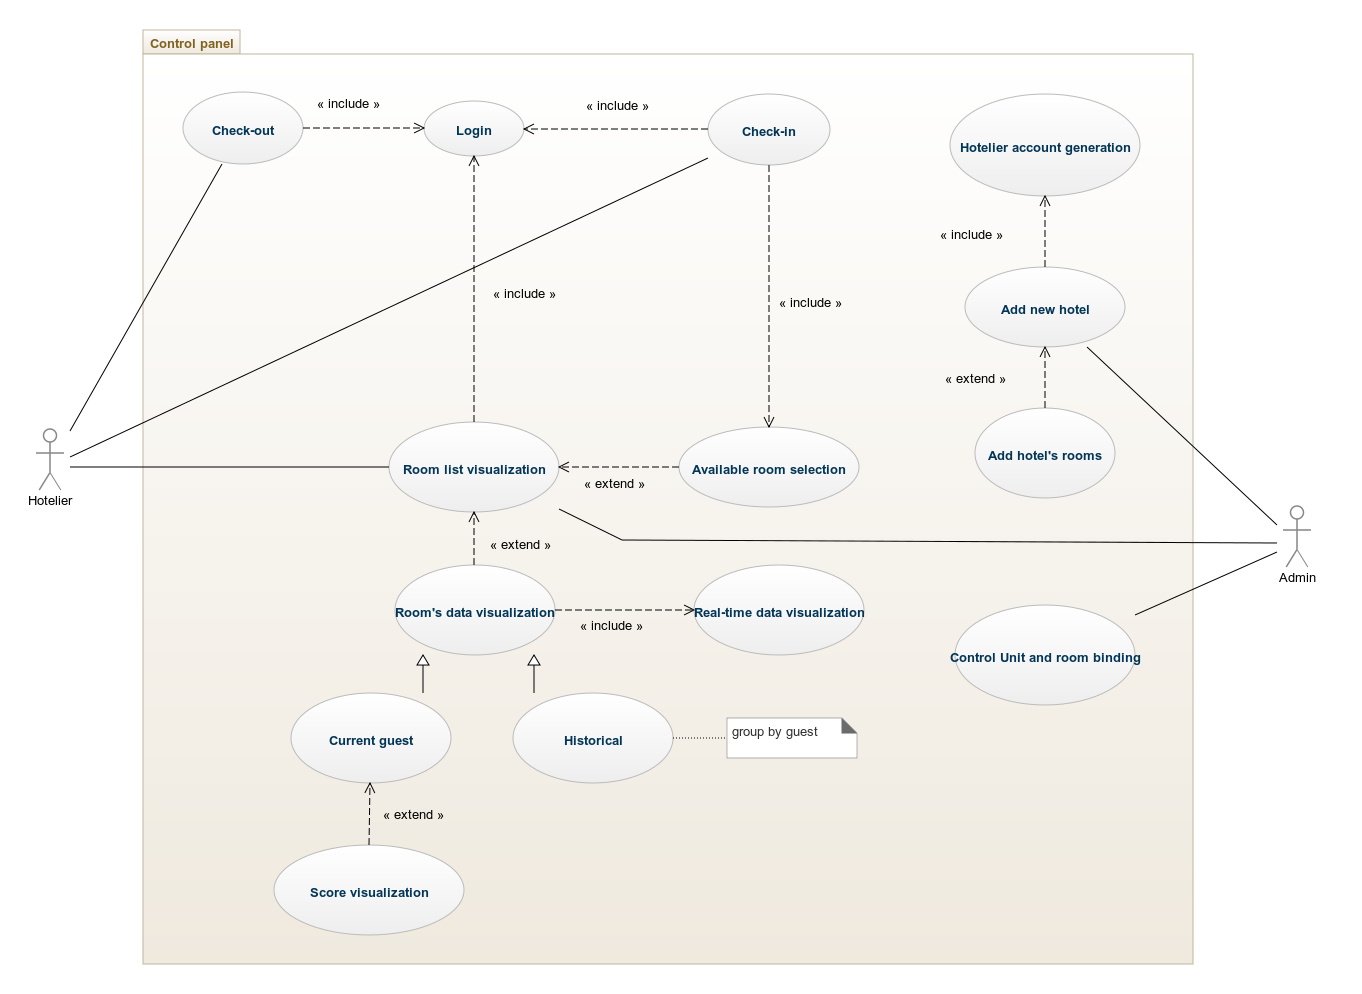
\includegraphics[width=\textwidth]{control-panel-usecase.png}
    \centering
    \caption[control-panel-usecase]{Schema dei casi d'uso del pannello di controllo.}
    \label{fig:cp-usecase}
\end{figure}

\begin{figure}[H]
    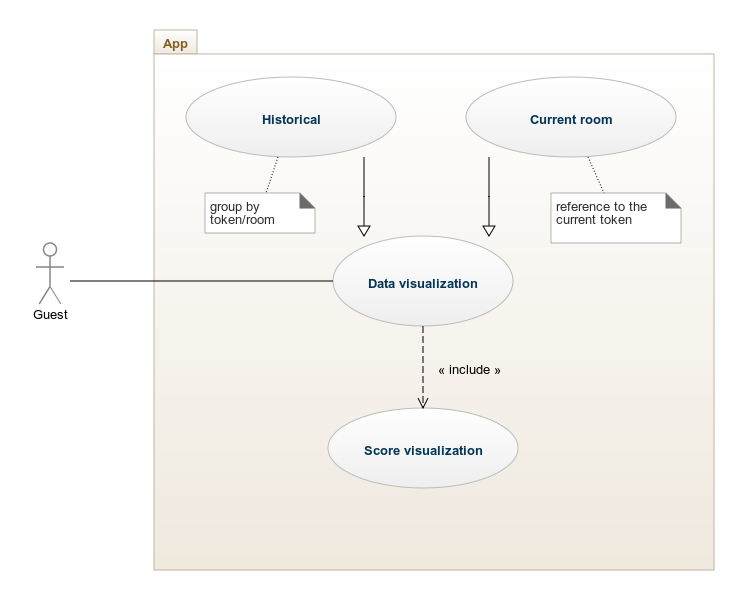
\includegraphics[width=0.8\textwidth]{app-use-case.png}
    \centering
    \caption[app-usecase]{Schema dei casi d'uso relativi all'applicazione lato ospite.}
    \label{fig:app-usecase}
\end{figure}

\begin{figure}[H]
    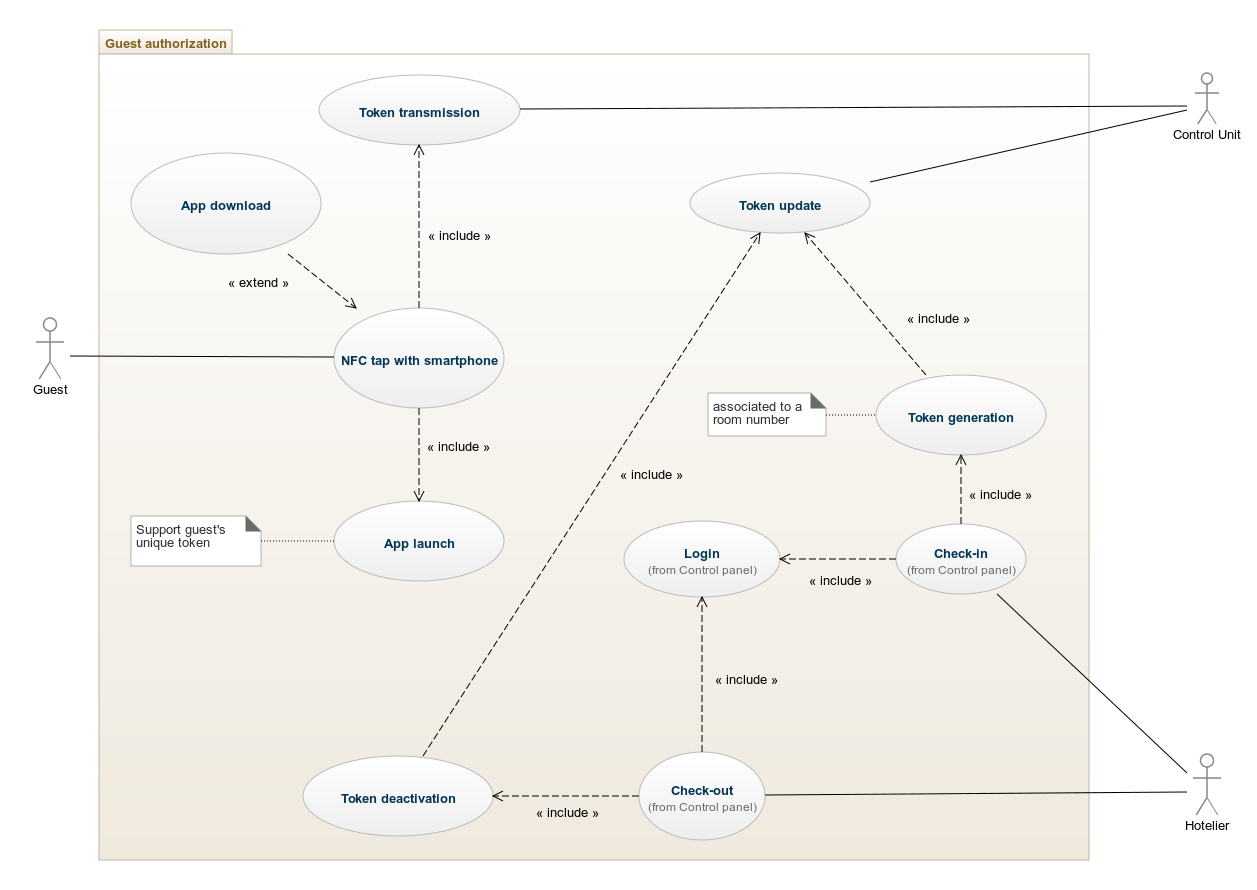
\includegraphics[width=\textwidth]{guest-authorization-use-case.png}
    \centering
    \caption[guest-authorization-usecase]{Schema dei casi d'uso del meccanismo di autorizzazione dell'ospite.}
    \label{fig:guest-authorization-usecase}
\end{figure}

\begin{figure}[H]
    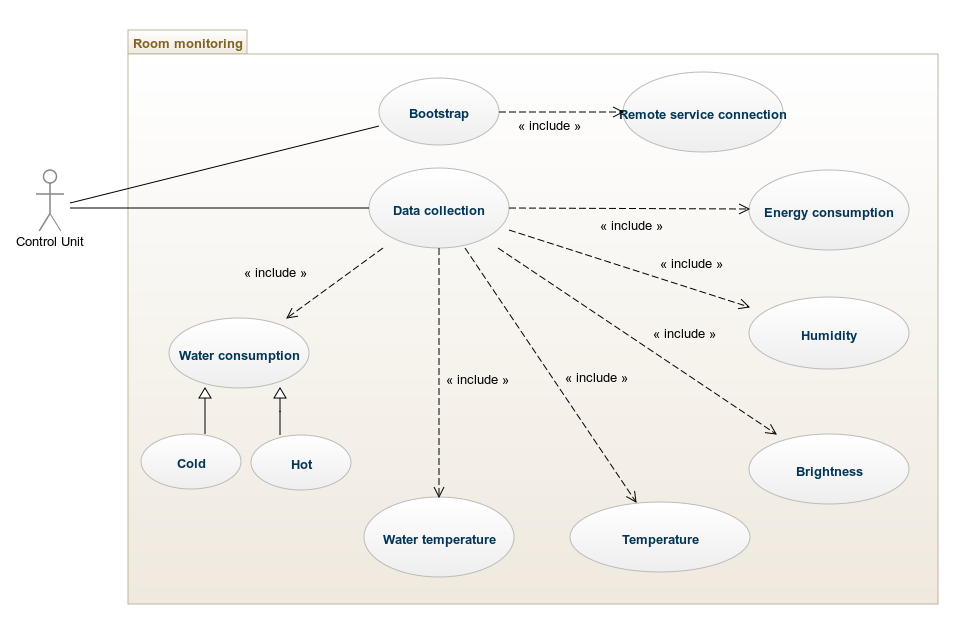
\includegraphics[width=\textwidth]{room-monitoring-use-case.png}
    \centering
    \caption[room-monitoring-usecase]{Schema dei casi d'uso relativi alla \textit{control unit}.}
    \label{fig:room-monitoring-usecase}
\end{figure}

\subsection{Sottodomini del problema}
Decomponiamo il nostro problema in 9 sottodomini (Figura \ref*{fig:subdomains}).
Un sottodominio (o un piccolo gruppo di questi) rappresenta un sotto-progetto indipendente con i propri requisiti, design e ciclo di sviluppo.

\begin{figure}[H]
    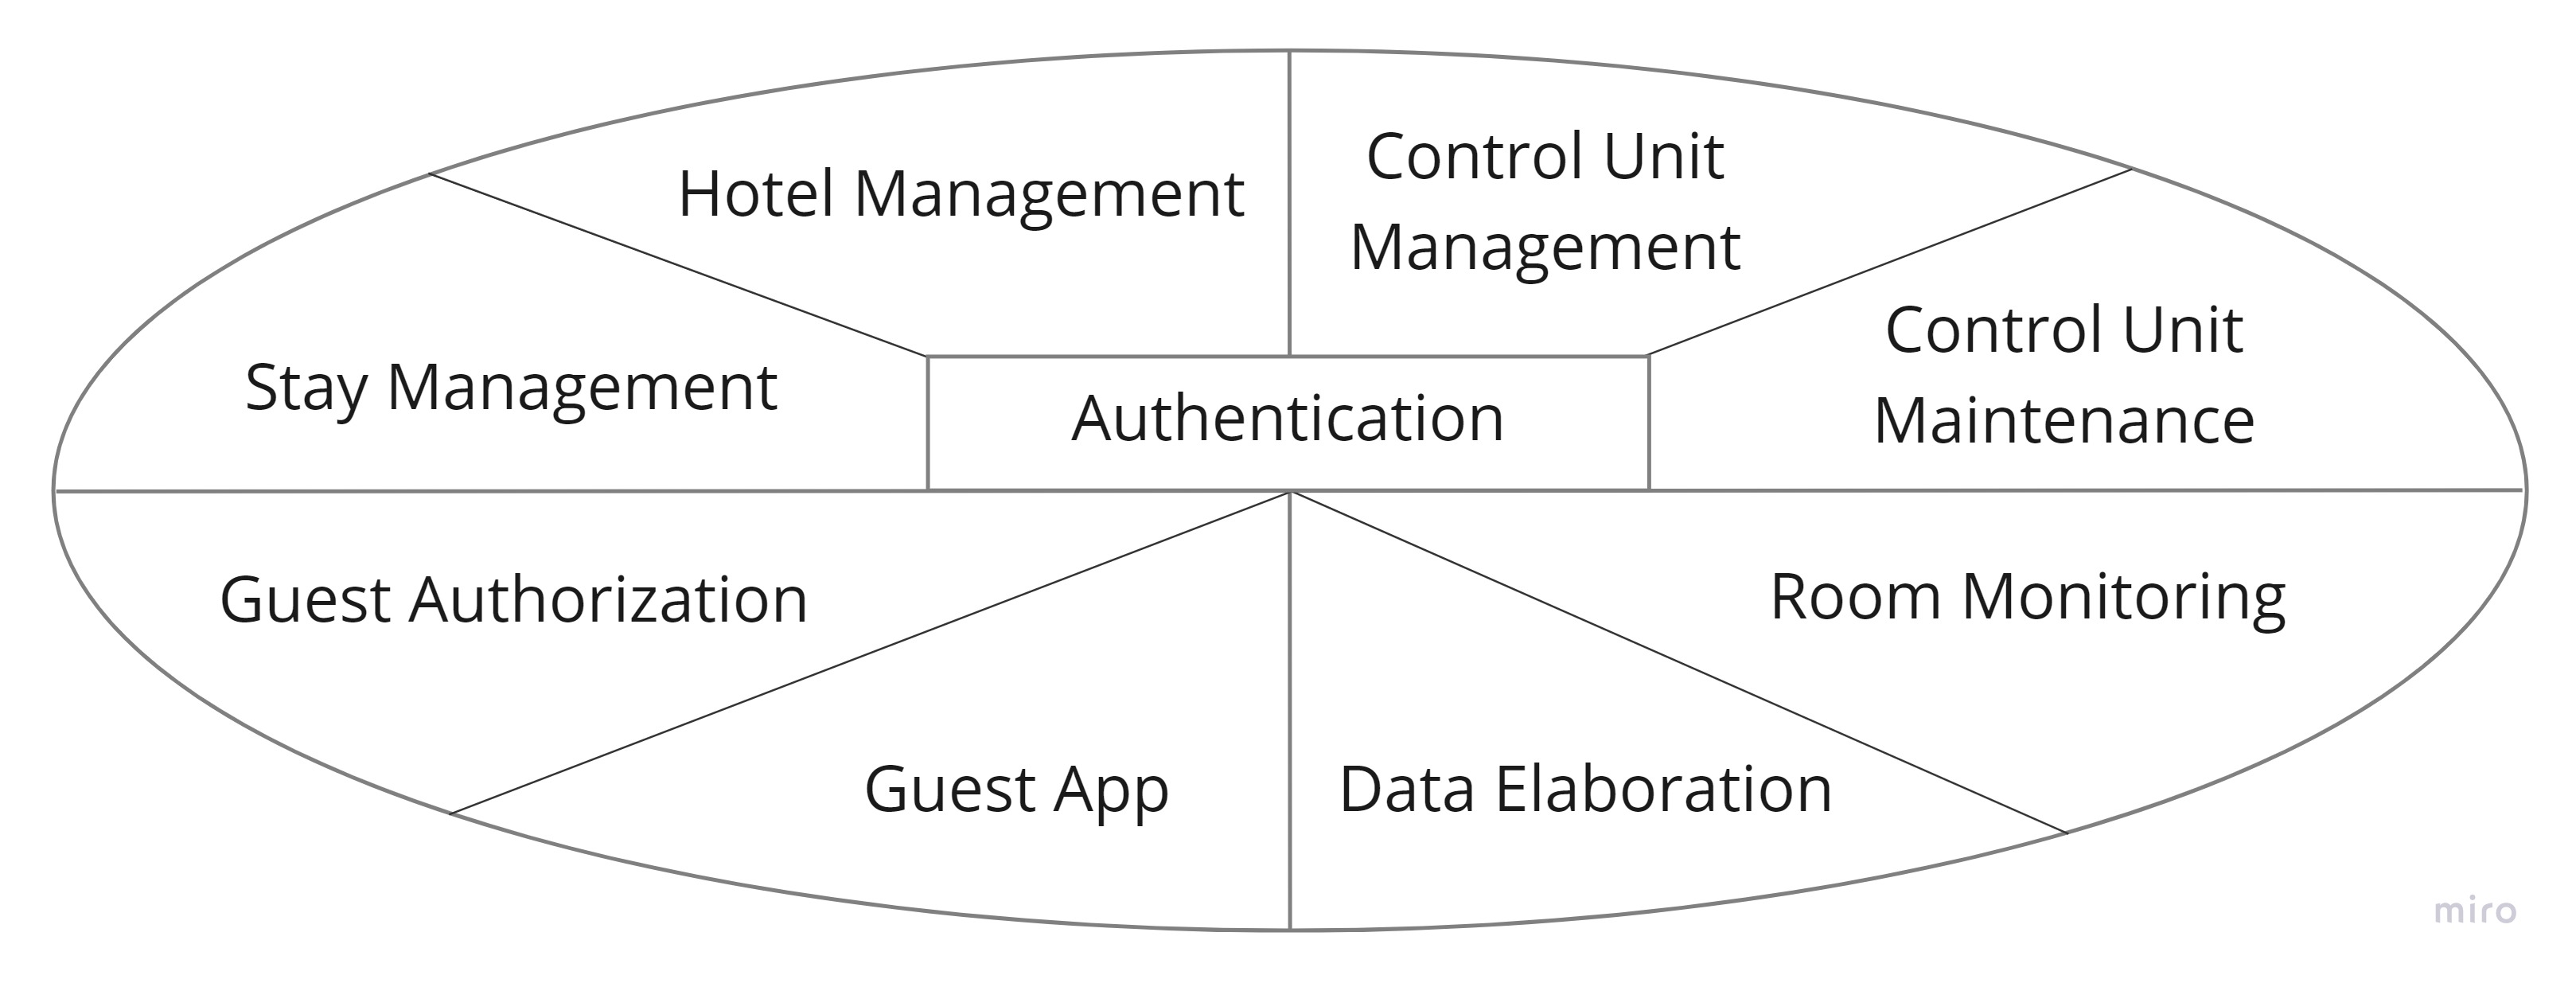
\includegraphics[width=\textwidth]{subdomains.jpg}
    \centering
    \caption[subdomains]{Sottodomini del sistema Ecotrip.}
    \label{fig:subdomains}
\end{figure}
\begin{itemize}
    \item \textit{Hotel Management}: comprende le funzionalità svolte dall'amministratore Ecotrip che riguardano la configurazione di nuovi hotel e relative camere.
    \item \textit{Stay Management}: comprende la gestione dei soggiorni con le funzioni di \textit{check-in} e \textit{check-out} da parte dell'hotelier.
    \item \textit{Authentication}: comprende sia l'autenticazione utenti quali amministratore Ecotrip e \textit{hotelier} richiesta per l'utilizzo dei servizi come \textit{Hotel} e \textit{Stay Management}, che la possibilità di registrare gli \textit{account} per gli \textit{hotelier}.
    \item \textit{Control Unit Management}: comprende la gestione delle centraline installate con la possibilità di verifica dello stato e di abbinamento alle camere.
    \item \textit{Control Unit Maintenance}: comprende il sistema per la manutenzione da remoto delle centraline installate.
    \item \textit{Room Monitoring}: comprende il sistema per il campionamento dei dati dai sensori della centralina e lo stoccaggio in un servizio cloud.
    \item \textit{Data Elaboration}: comprende il sistema per il calcolo della stima dei consumi C02 e del punteggio "sostenibilità" relativo ai soggiorni, a partire dai dati collezionati.
    \item \textit{Guest Authorization}: include il processo di generazione del \textit{token} per un nuovo soggiorno ed il suo trasferimento alla centralina e successivamente allo smartphone mediante \textit{transponder} NFC, permettendo così all'ospite di accedere ai dati del suo soggiorno.
    \item \textit{Guest App}: include la visualizzazione dei dati del soggiorno tramite applicativo fruibile dagli ospiti, inoltre implementa gli aspetti di \textit{gamification}.
\end{itemize}

\subsection{Requisiti di sistema}

Dettagliamo di seguito i requisiti di sistema funzionali suddivisi per i diversi sottodomini del sistema Ecotrip.
Successivamente specifichiamo i requisiti non funzionali.

\begin{itemize}
    \item Requisiti funzionali

    \begin{itemize}
        \item Authentication
        \begin{itemize}
            \item Autenticazione utenti con email e password
            \item Registrazione nuovi utenti
            \item Ruoli previsti: amministratori ecotrip e albergatori
        \end{itemize}
    \end{itemize}

    \begin{itemize}
        \item Room Monitoring
        \begin{itemize}
            \item Raccolta dati con campionamento ogni secondo da diversi sensori
            \begin{itemize}
                \item Rilevazione del consumo energetico con sensore di corrente
                \item Rilevazione del consumo di acqua tramite due flussometri
                \item Rilevazione della temperatura di acqua calda / fredda tramite due sensori di temperatura
                \item Rilevazione dello stato delle tende (aperte/chiuse) della stanza attraverso un sensore di luminosità installato su ogni finestra
                \item Rilevazione della temperatura della stanza mediante un sensore di temperatura ambientale
                \item Rilevazione della percentuale di umidità della stanza tramite un sensore di umidità ambientale
            \end{itemize}
            \item Identificazione presenza ospite all'interno della stanza (opzionale)
            \item Aggregazione dati campionati ogni 5 secondi
            \begin{itemize}
                \item Calcolo del consumo energetico
                \item Calcolo del consumo di acqua
            \end{itemize}
            \item Invio ogni 5 secondi dei dati rilevati ed aggregati a piattaforma cloud
        \end{itemize}
    \end{itemize}

    \begin{itemize}
        \item Guest Authorization
        \begin{itemize}
            \item Generazione token univoco, firmato e verificabile al checkin dell'ospite contenete identificativi di hotel, stanza e pernottamento
            \item Sincronizzazione su centralina del token generato in remoto
            \item Controllo sensore NFC su centralina per trasferire il token a dispotivo mobile
            \item Il tag NFC deve funzionare in modo da avviare sullo smartphone la web app Ecotrip senza azione dell'utente, 
                    ma solo all'avvicinamento del dispositivo al tag
        \end{itemize}
    \end{itemize}

    \begin{itemize}
        \item Control Unit Management
        \begin{itemize}
            \item Configurazione da parte degli amministratori Ecotrip di nuove centraline installate assegnando identificativo di hotel e stanza
            \item Verifica dello stato di funzionamento da remoto da parte degli amministratori Ecotrip
        \end{itemize}
    \end{itemize}

    \begin{itemize}
        \item Control Unit Maintenance
        \begin{itemize}
            \item Accesso da remoto a centralina installata da parte agli amministratori Ecotrip
            \item Aggiornamento automatico del software della centralina
        \end{itemize}
    \end{itemize}

    \begin{itemize}
        \item Hotel Management
        \begin{itemize}
            \item Accesso a pannello di controllo riservato solo agli amministratori ecotrip
            \item Gestione completa degli hotel con informazioni quali: identificativo, nome, indirizzo e costo dell'energia nei termini di CO2/Kilowatt
            \item Possibilità di creare l'account dell'albergatore per un hotel
            \item Gestione completa delle camere di un'hotel con informazioni quali: identificativo e numero
        \end{itemize}
    \end{itemize}

    \begin{itemize}
        \item Stay Management
        \begin{itemize}
            \item Accesso a pannello di controllo riservato agli amministratori ecotrip ed all'albergatore proprietario dell'hotel
            \item Visualizzazione dei pernottamenti suddivisi per camera
            \item Per ogni camera possibilità di eseguire check-in e check-out di un ospite
            \item Visualizzazione del punteggio "sostenibilità" del pernottamento con relativo consumo totale di CO2
            \item Visualizzazione dei consumi istantanei di una camera
        \end{itemize}
    \end{itemize}

    \begin{itemize}
        \item Data Elaboration
        \begin{itemize}
            \item Calcolo della CO2 a partire dai dati di un pernottamento
            \item Algoritmo per il calcolo del punteggio "sostenibilità" di un pernottamento a partire dalla CO2 generata e considerando il comportamento tenuto dall'ospite:
            \begin{itemize}
                \item uso eccessivo di acqua
                \item uscire dalla camera lasciando il condizionatore accesso e le tende aperte di giorno  
            \end{itemize}
        \end{itemize}
    \end{itemize}

    \begin{itemize}
        \item Guest App
        \begin{itemize}
            \item Avvio automatico con avvicinamento del dispositivo mobile al tag NFC
            \item Visualizzazione dei dati del pernottamento corrente: informazioni generali, consumo CO2 e "punteggio sostenibilità"
            \item Visualizzazione dei dati dei pernottamenti passati
        \end{itemize}
    \end{itemize}
    
    \item Requisiti non funzionali
    \begin{itemize}
        \item Garantire privacy per gli ospiti sia per quanto riguarda la scelta dei meccanismi/sensori utilizzati dalla centralina, 
                sia per quanto concerne la possibilità che qualcuno possa accedere ai dati non propri (esempio ospiti che accedono a dati di altri ospiti)
        \item Scalabilità del sistema cloud all'occorrenza, sia per quanto concerne la ricezione ed elaborazione dei dati che per gli ospiti connessi
    \end{itemize}
\end{itemize}
%
%----------------------------------------------------------------------------------------
%	PROGETTAZIONE
%----------------------------------------------------------------------------------------

\section{Progettazione}
Una volta chiarificati tutti i requisiti ed i desiderata del cliente, si è passati alla fase di progettazione. Inizialmente si è preferito astrarre dalle tematiche di "basso livello" dando priorità alla definizione di tutti i servizi necessari per il corretto funzionamento del sistema. Nello specifico si parla di microservizi, infatti ogni componente software da sviluppare modella un insieme specifico di concetti, precedentemente identificati nei 9 sottodomini. Un aspetto di cruciale importanza è definire a monte le modalità di interazione tra i vari servizi. Per ognuna di queste è necessario specificare il "fornitore" (\textit{upstream}) ed il "consumatore" (\textit{downstream}), così da stabilire una dipendenza tra le coppie di servizi che vincoli una delle parti ad adattarsi alle regole operative dell'altra.

\begin{figure}[H]
    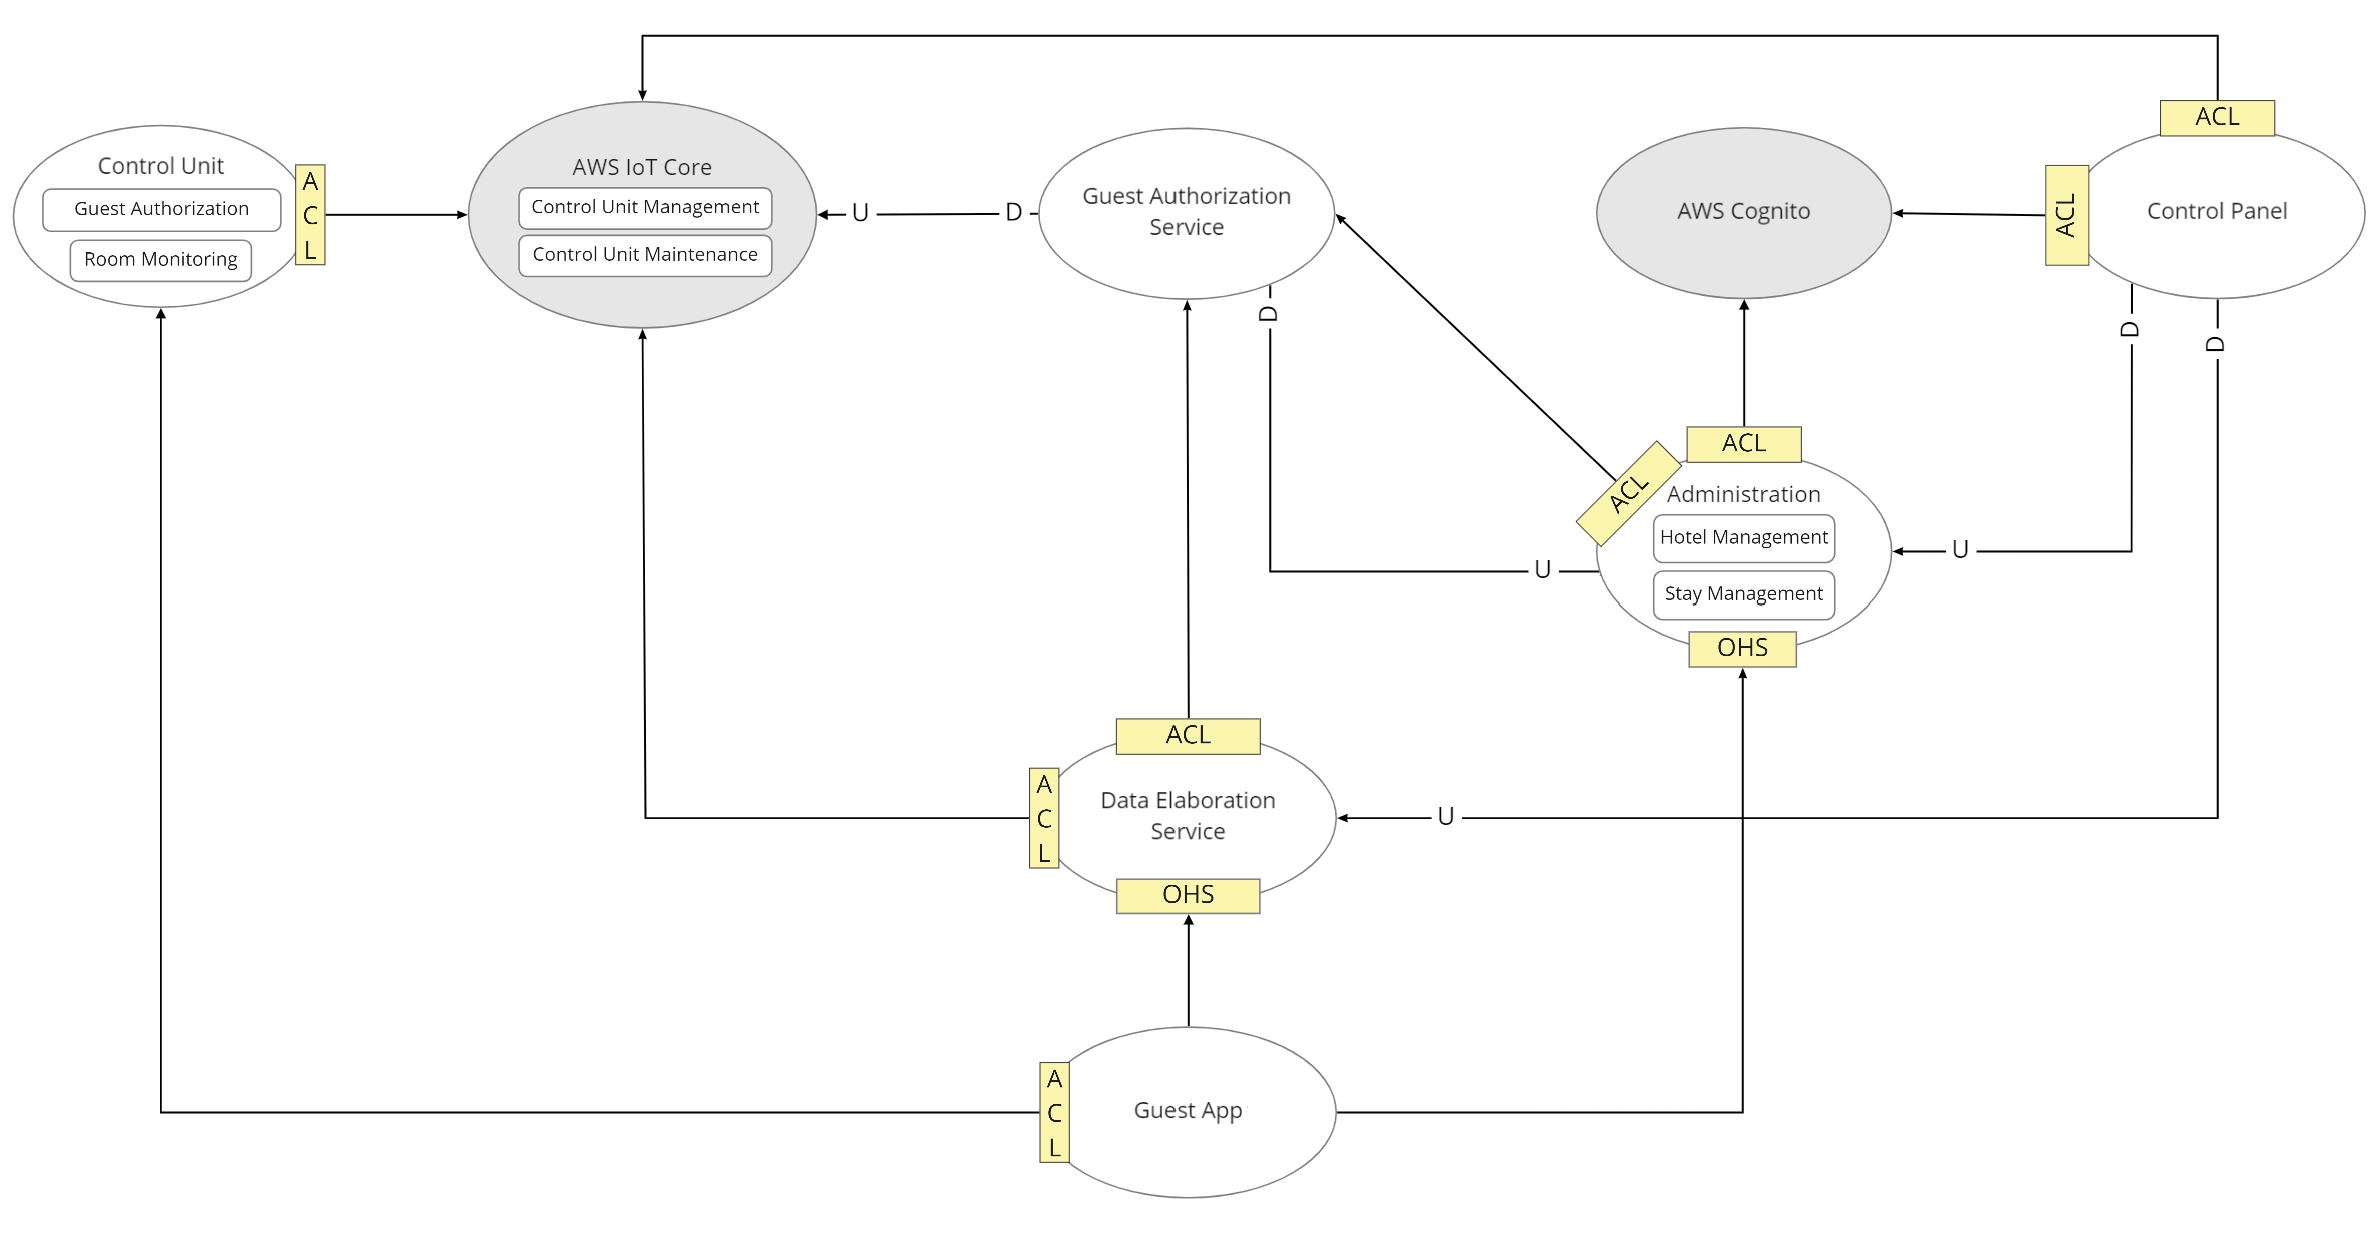
\includegraphics[width=\textwidth]{context-map.png}
    \centering
    \caption[contextmap]{Schema dei microservizi che compongono Ecotrip}
    \label{fig:contextmap}
\end{figure}

Le componenti del sistema Ecotrip (Figura \ref{fig:contextmap}) possono essere schematizzate in:
\begin{itemize}
    \item \textbf{Administration}: servizio che modella  i concetti e implementa le funzionalità di gestione degli hotel (\textit{Hotel Management}) e dei pernottamenti (\textit{Stay Management}).  Entrambe queste API necessitano di verificare l'autenticità delle richieste, per questo Administration dipende sia da AWS Cognito e che da Guest Authorization Service, il quale genera i \textit{token} usati da Guest App per eseguire le richieste. Queste due dipendenze in realtà non rappresentano connessioni con i servizi remoti in quanto le verifiche possono essere eseguite localmente ad Administration, tuttavia il processo di validazione è vincolato alle tecnologie usate dai rispettivi servizi. La comunicazione verso i servizi di AWS Cognito e Guest Authorization sarà regolamentata da opportuni \textit{adapter} (ACL) che consentono di convertire, sia in entrata che in uscita, i concetti di dominio esterni in quelli interni al servizio stesso.  
    Poiché è richiesto che il pannello di controllo sia fruibile via web, si applica il \textit{backend-for-frontend pattern}: Administration si occuperà di fornire una RESTful API ad uso del \textit{frontend} che sarà descritto in seguito.
    Si è quindi evitata una logica a microservizi pura in quanto:
    \begin{itemize}
        \item il ciclo di vita può essere unito in modo da avere un unico deployment su unica infrastruttura riducendo i costi di fornitura del servizio;
        \item Hotel Management avrà un numero di richieste sempre molto basso e lo \textit{scaling} del servizio può essere dimensionato pensando solamente a Stay Management.
    \end{itemize}
    L'alternativa a questa strategia è di separare i due servizi e progettarli con paradigma totalmente \textit{serverless}, che renda i costi del servizio proporzionali all'utilizzo. Questa modalità però dipende strettamente dai servizi offerti dal \textit{cloud provider} e richiederebbe uno studio più approfondito dello stesso, cosa che non è possibile affrontare in questa sede.
    \item \textbf{AWS Cognito}: rappresenta il sottodominio relativo all'autenticazione, cioè tutte le funzionalità che consento di gestire gli \textit{account} degli amministratori di sistema e degli \textit{hotelier}, che può essere demandato in \textit{out-sourcing}. Una possibile soluzione può essere Amazon AWS Cognito.
    \item \textbf{Control Panel}: realizza la logica di business \textit{frontend} dei sottodomini Administration e Authentication, nella pratica si andrà a realizzare una \textit{web app} sfruttando il framework React.js. Questa delegherà l'autenticazione e la gestione degli account creati ad AWS Cognito. Inoltre, il pannello di controllo risultante dovrà permettere di visualizzare sia lo stato dalle centraline che i dati prodotti da queste. Ciò comporta la creazione di un collegamento tra il Control Panel ed i servizi AWS IoT Core e Data Elaboration Service.
    \item \textbf{AWS IoT Core}: include i sottodomini Control Unit Management, Control Unit Maintenance e lo \textit{storage cloud} dei dati generati da Room Monitoring. Come per l'autenticazione, la sua implementazione può essere delegata a un fornitore esterno, nel caso specifico si è scelto l'omonimo servizio di amazon AWS IoT Core. Quest'ultimo dispone di un pannello di controllo con cui poter agevolmente eseguire tutti i \textit{task} richiesti, per esempio permette di abbinare le centraline alle stanze attraverso \textit{tagging}. Infine, tramite un'apposita Rest API, per ogni centralina si è in grado di ottenere i dati caricati, verificarne lo stato ed inviare dei comandi da remoto: funzionalità che può essere sfruttata per inviare il token di un ospite.
    \item \textbf{Guest Authorization}: realizza funzionalità che possono essere circoscritte in due sistemi distinti. Il primo è Guest Authorization Service, il quale si occupa della generazione del \textit{token}, a seguito della creazione di un nuovo soggiorno (eventi di \textit{check in} e \textit{check out}) da parte del servizio di Stay Management, e del suo invio verso la centralina tramite AWS IoT Core. Il secondo sistema verrà incluso come modulo all'interno del software della centralina.
    \item \textbf{Control Unit}: rappresenta il software installato sulla centralina, il quale si compone di due moduli, il primo (Room Monitoring) si occupa del monitoraggio dei consumi, mentre il secondo (Guest Authorization) è dedicato alla gestione del \textit{transponder NFC}. La Control Unit oltre a ricevere gli aggiornamenti di stato da AWS IoT Core, vi inoltra i dati raccolti dai sensori. Come fatto per Administration, anche in questo caso si è evitato di creare due software indipendenti al fine di avere lo stesso ciclo di vita e un unico \textit{deployment} che possa semplificare le attività di configurazione e manutenzione della centralina.
    \item \textbf{Guest App}: realizza un applicativo lato \textit{frontend} che comunica con la Control Unit per ottenere il \textit{token} da presentare al servizio di Data Elaboration per accedere ai dati del pernottamento.
\end{itemize}

Di seguito viene proposto un approfondimento su ogni componente appena elencata.

\subsection{Control Unit}
Nel caso specifico della centralina la fase di progettazione coinvolge sia la componente \textit{hardware} che quella \textit{software}. L'elemento \textit{core} del prototipo è una scheda \textit{raspberry pi 4B} alla quale sono connessi i sensori precedentemente citati nella sezione dei requisiti. Data la finalità prototipale e le tempistiche ristrette si predilige l'acquisto di un set di sensori che siano disponibili nell'immediato, preferibilmente digitali e con un supporto software adeguato. Ovviamente, di questi si verificherà anche l'accuratezza nonostante non sia ritenuto un aspetto fondamentale durante questa fase di progetto. 

\subsubsection{Hardware}
Dopo un'attenta fase di ricerca e un confronto tra le diverse soluzioni, si opta per l'acquisto di un determinato set di sensori, presentato e approfondito nella sezione corrente. Di ciascuno verrà fornita una breve descrizione che include le caratteristiche tecniche principali, mentre i dettagli relativi alla componente software saranno trattati nella sezione successiva.\newline\newline
%
\textbf{ICQUANZX PN532 NFC}\footnote{Link al venditore: \href{https://www.amazon.it/ICQUANZX-Communication-Arduino-Raspberry-Android/dp/B07VT431QZ/}{https://www.amazon.it/ICQUANZX}}: modulo di trasmissione altamente integrato per la comunicazione NFC (Near Field Communication) a 13.56 MHz. Il sensore è dotato di un interruttore con il quale è possibile cambiare la modalità scegliendo tra I2C, SPI e UART. Inoltre, il modulo supporta la lettura/scrittura RFID e possiede 4 fori di montaggio da 3mm. 
    
\begin{table}[H]
    \centering
    \begin{tabular}{|l|l|}
    \hline
    \textbf{Caratteristica}     & \textbf{Descrizione}                      \\ \hline        Protocollo di comunicazione                   & I2C\footnote{Per dettagli: \url{https://www.i2c-bus.org/}}, SPI and HSU (High Speed UART)                                                                                                                     \\ \hline
    Supporto RFID                                 & \begin{tabular}[c]{@{}l@{}}modalità in lettura o scrittura:\\   - Mifare 1k, 4k, Ultralight, and DesFire cards\\   - ISO/IEC 14443-4 card\end{tabular} \\ \hline
    Distanza di comunicazione                     & 5cm$\sim$7cm (PCB Antenna)                                                                                                                             \\ \hline
    Virtualizzazione                              & può funzionare come una carta virtuale                                                                                                                 \\ \hline
    Dimensioni                                    & 43mm x 41mm x 4mm                                                                                                                                          \\ \hline
    \end{tabular}
    \caption{\label{pn532-features}Caratteristiche principali del modulo PN-532.}

\end{table}

La modalità di funzionamento determina anche la configurazione a livello di circuito (alimentazione).
\begin{table}[H]
    \centering
    \begin{tabular}{|c|c|}
    \hline
    \textbf{Interfaccia} & \textbf{Valore}                            \\ \hline
    VCC                & 3.3V$\sim$5V                              \\ \hline
    I2C/UART           & 3.3V$\sim$24V TTL                         \\ \hline
    SPI                & 3.3V TTL con 100 ohm di resistenza \\ \hline
    \end{tabular}
    \caption{\label{pn532-modalities}Modalità di funzionamento del modulo PN-532.}
\end{table}

\begin{figure}[H]
    \begin{center}
        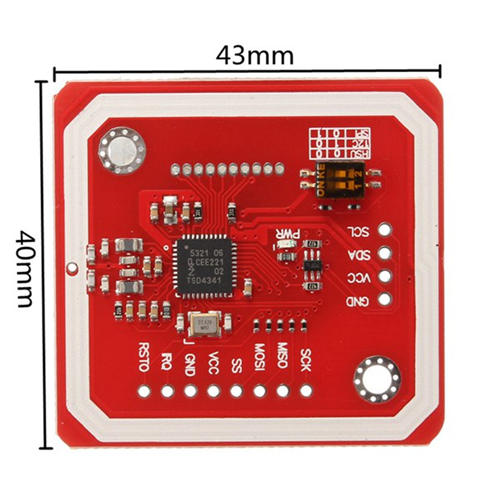
\includegraphics[width=0.35\textwidth]{images/sensors/pn532.png}
    \end{center}
    \caption{\label{pn532}Modulo PN532}
\end{figure}

Nel caso si voglia comunicare con il sensore tramite l'interfaccia I2C, è necessario impostare gli interruttori rispettivamente a \texttt{ON} e \texttt{OFF} (Tabella \ref*{tb-PN532-interfaces}). Inoltre la connessione alla scheda richiede l'utilizzo di 4 pin (Tabella \ref*{tb-PN532-conn-schema}). Una volta connesso il modulo sarà identificato dalla scheda con l'indirizzo \texttt{0x24}.
\begin{table}[H]
    \centering
    \begin{tabular}{|l|l|l|}
    \hline
    \textbf{Interfaccia} & \textbf{Canale 1} & \textbf{Canale 2} \\ \hline
    HSU                  & OFF               & OFF               \\ \hline
    I2C                  & ON                & OFF               \\ \hline
    SPI                  & OFF               & ON                \\ \hline
    \end{tabular}
    \caption{\label{tb-PN532-interfaces}Schema di collegamento modulo PN532.}
\end{table}

\begin{table}[H]
    \centering
    \begin{tabular}{|l|l|l|}
    \hline
    \multicolumn{1}{|c|}{\textbf{Module PCB}} & \multicolumn{1}{c|}{\textbf{Desc}} & \multicolumn{1}{c|}{\textbf{GPIO Header Pins}} \\ \hline
    GND                                       & Ground                             & P1-6                                          \\ \hline
    SDA                                       & I2C SDA                            & P1-03                                          \\ \hline
    SCL                                       & I2C SCL                            & P1-05                                          \\ \hline
    VCC                                       & 3.3V                               & P1-01                                          \\ \hline
    \end{tabular}
    \caption{\label{tb-PN532-conn-schema}Schema di collegamento modulo PN532.}
\end{table}

\begin{figure}[H]
    \begin{center}
      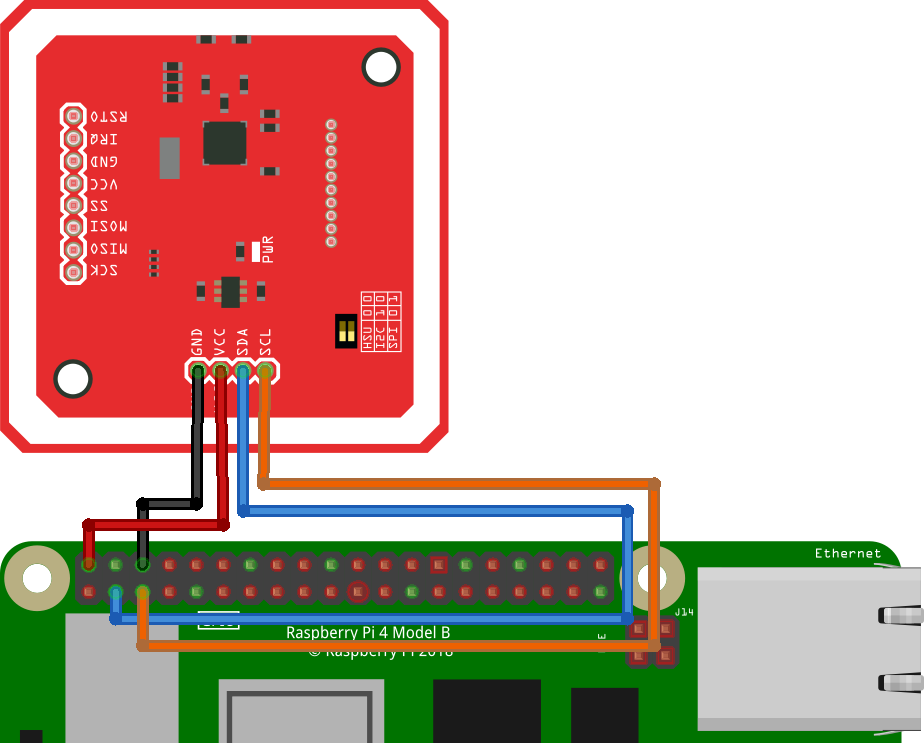
\includegraphics[width=0.6\textwidth]{images/sensors/pn532-fritzing.png}
    \end{center}
    \caption{\label{pn532-diagram}Diagramma Fritzing del modulo PN532 (connessione I2C).}
\end{figure}
    
    
\textbf{GY-302 BH1750}\footnote{Link al venditore: \href{https://www.amazon.it/AZDelivery-Sensore-Intensità-Luminosità-Raspberry/dp/B07NLL4SCB}{https://www.amazon.it/AZDelivery-BH170}}: sensore digitale per il rilevamento della luminosità ambientale basato sull'interfaccia bus I2C; internamente monta un ADC. Le caratteristiche complete del sensore possono essere visionate consultando la pagina del \href{https://www.mouser.com/datasheet/2/348/bh1750fvi-e-186247.pdf}{\textit{datasheet}}. 

\begin{table}[H]
    \centering
    \begin{tabular}{|l|l|}
    \hline
    \textbf{Caratteristica}     & \textbf{Descrizione}                      \\ \hline    Alimentazione               & 3$\sim$5V                                 \\ \hline
    Protocollo di comunicazione & I2C                                       \\ \hline
    Output                      & segnale in uscita digitale (ADC build-in) \\ \hline
    Accuratezza                 & precisione elevata, vicino a 1 Lu         \\ \hline
    Data range                  & 0$\sim$65535                              \\ \hline
    Dimensioni                  & 13.9 x 18.5 mm                           \\ \hline
    \end{tabular}
    \caption{\label{bh1750-features}Caratteristiche principali del modulo BH1750.}
\end{table}
%
\begin{figure}[H]
    \begin{center}
      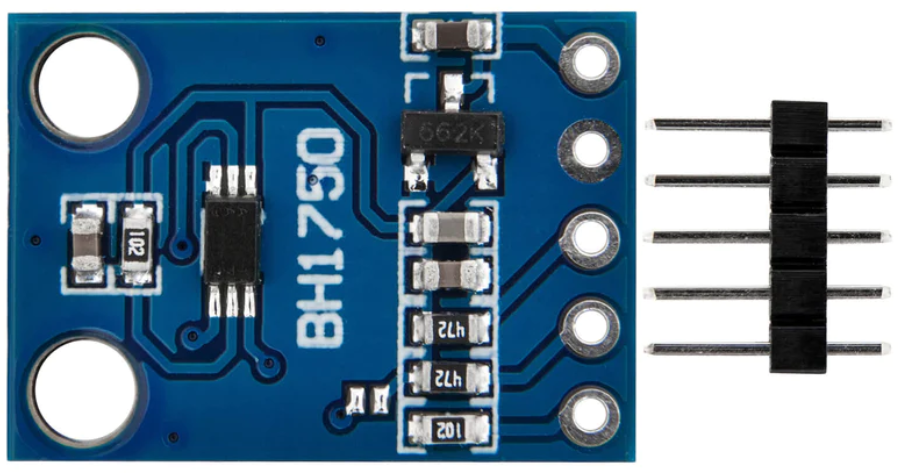
\includegraphics[width=0.35\textwidth]{images/sensors/bh1750.png}
    \end{center}
    \caption{Modulo BH1750}
\end{figure}
%
Il sensore può essere collegato al Raspberry Pi semplicemente sfruttando 4 collegamenti (o meglio 4 pin GPIO della scheda come descritto in Tabella \ref*{tb-BH1750-conn-schema}). Una volta realizzato il circuito (Figura \ref*{bh1750-diagram}), il comando \texttt{i2cdetect} restituirà in input l'indirizzo del sensore, che nel caso specifico equivale a \texttt{0x23}.
%
\begin{table}[H]
    \centering
    \begin{tabular}{|l|l|l|}
    \hline
    \multicolumn{1}{|c|}{\textbf{Module PCB}} & \multicolumn{1}{c|}{\textbf{Desc}} & \multicolumn{1}{c|}{\textbf{GPIO Header Pins}} \\ \hline
    GND                                       & Ground                             & P1-14                                          \\ \hline
    ADD                                       & Address select                     & P1-14                                          \\ \hline
    SDA                                       & I2C SDA                            & P1-03                                          \\ \hline
    SCL                                       & I2C SCL                            & P1-05                                          \\ \hline
    VCC                                       & 3.3V                               & P1-01                                          \\ \hline
    \end{tabular}
    \caption{\label{tb-BH1750-conn-schema}Schema di collegamento modulo BH1750.}
\end{table}

\begin{figure}[H]
    \begin{center}
      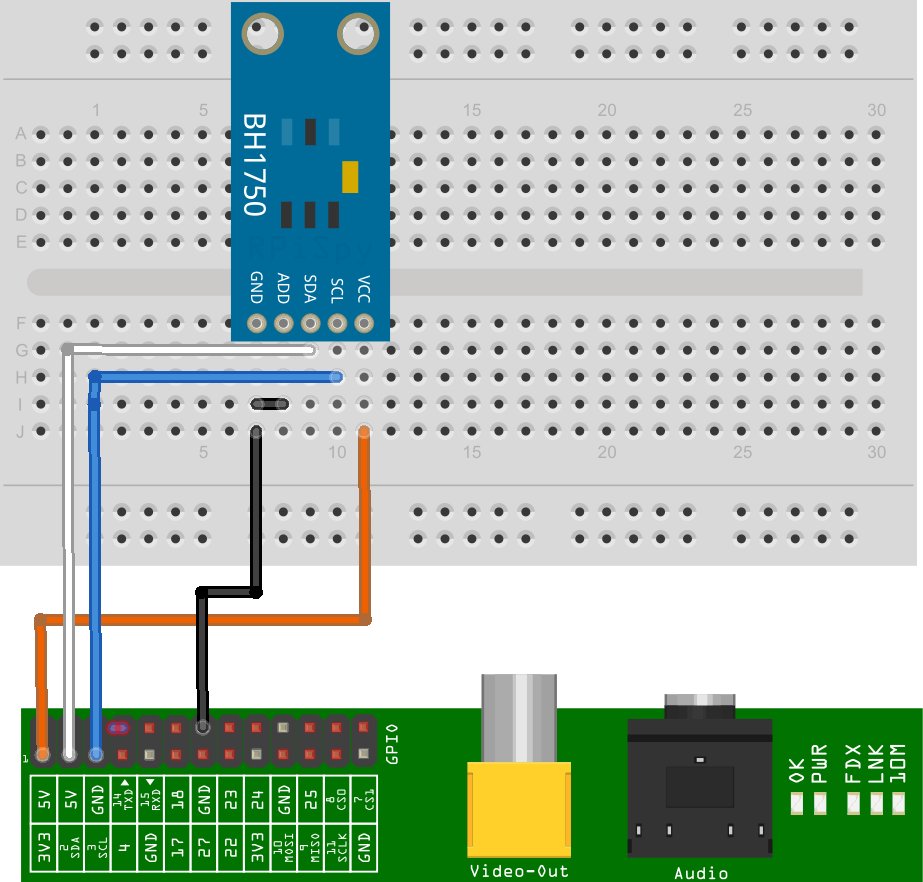
\includegraphics[width=0.6\textwidth]{images/sensors/BH1750-fritzing.png}
    \end{center}
    \caption{\label{bh1750-diagram}Diagramma Fritzing del modulo BH1750.}
\end{figure}

%
\textbf{ACS712 - 20A}\footnote{Link al venditore: \href{https://www.amazon.it/AZDelivery-corrente-sensore-Current-Raspberry/dp/B0736DYV3W?th=1}{https://www.amazon.it/AZDelivery-ACS712}}: sensore di corrente usato per misurare una corrente AC o DC in un range di ±20A con un errore di 1.5\% a T = 25 °C. Il sensore è composto da due parti, un collegamento per il chip del sensore, e l'altra parte con due connettori a morsettiera per la misurazione della corrente.
Il sensore utilizza l'effetto Hall per rilevare la corrente che lo attraversa. La corrente che fluisce attraverso il sensore genera un campo magnetico che viene rilevato dal sensore e convertito in una tensione analogica proporzionale. Questo modulo emette tensione analogica (0 ÷ 5 V) in base al flusso di corrente nel filo su cui viene eseguita la misurazione.
%
\begin{table}[H]
    \centering
    \begin{tabular}{|l|l|}
    \hline
    \textbf{Caratteristica} & \textbf{Descrizione}                                \\ \hline
    Alimentazione           & 5V                                                  \\ \hline
    Tensione in uscita      & metà di quella di allimentazione (2.5V se Vcc = 5V) \\ \hline
    Output                  & segnale in uscita digitale (ADC build-in)           \\ \hline
    Dimensioni              & 89.9 x 59.9 x 20.1 mm                               \\ \hline
    \end{tabular}
    \caption{\label{acs712-features}Caratteristiche principali del modulo ACS712.}
\end{table}

\begin{figure}[H]
    \begin{center}
      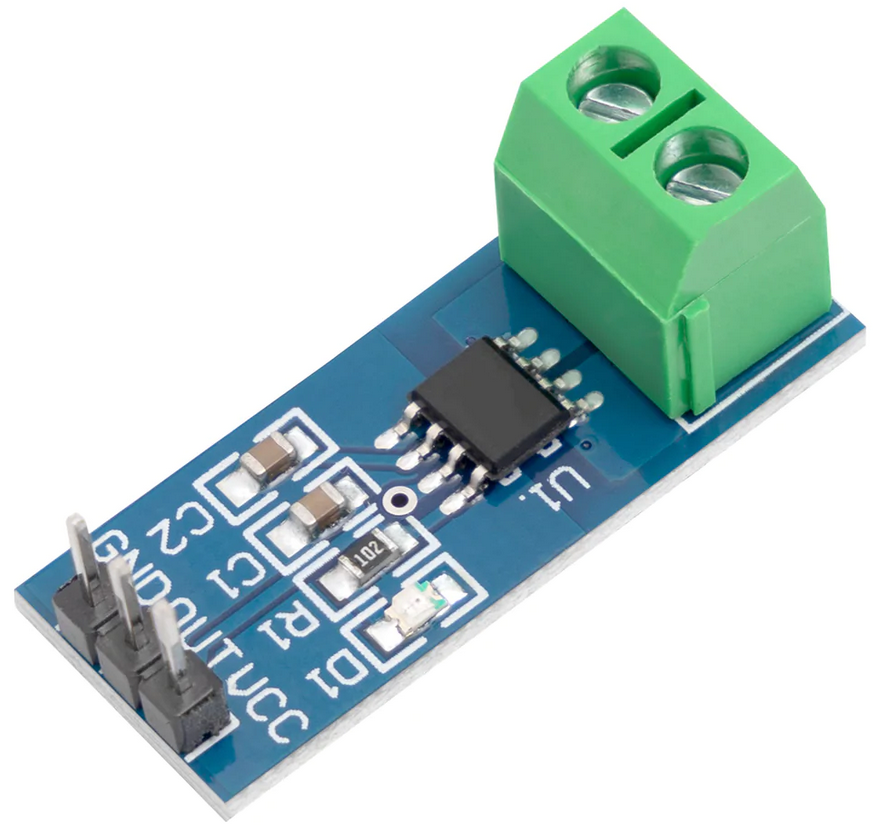
\includegraphics[width=0.35\textwidth]{images/sensors/acs712.png}
    \end{center}
    \caption{Modulo ACS712}
\end{figure}

\textbf{DHT22}\footnote{Link al venditore: \href{https://www.amazon.it/AZDelivery-temperatura-circuito-Raspberry-gratuito/dp/B078SVZB1X/ref=sr_1_6?keywords=dht22&qid=1673890614&sr=8-6&th=1}{https://www.amazon.it/AZDelivery-DHT22}}: sensore di umidità/temperatura relativa che emette un segnale digitale. Utilizza un sensore di umidità capacitivo e un termistore per misurare l'aria circostante. Nello specifico, la componente di umidità è costituita da un substrato di trattenimento che assorbe il vapore acqueo, andando ad aumentare la conduttività di due elettrodi posti agli estremi. Mentre la parte di rilevamento della temperatura del dispositivo è costituita da un sensore di temperatura NTC, cioè un termistore la cui resistenza diminuisce con l'aumentare della temperatura. Infine, c'è un piccolo PCB con un IC (circuito integrato) che esegue la conversione da analogico a digitale ed emette la coppia di valori (umidità e temperatura).

\begin{table}[H]
    \centering
    \begin{tabular}{|l|l|}
    \hline
    \textbf{Caratteristica} & \textbf{Descrizione}               \\ \hline
    Alimentazione           & 3$\sim$5V                          \\ \hline
    Tensione operativa max  & 2.5mA max                          \\ \hline
    Range umidità           & 0\% - 100\%  (accuratezza 2 - 5\%) \\ \hline
    Range di temperatura    & -40°C - 125°C (accuratezza ±0.5°C) \\ \hline
    Freq. di campionamento  & 0.5Hz (lettura ogni 2s)            \\ \hline
    Dimensioni              & 15 x 38 x 9 mm                     \\ \hline
    \end{tabular}
    \caption{\label{DHT22-features}Caratteristiche principali del modulo DHT22.}
\end{table}

\begin{figure}[H]
    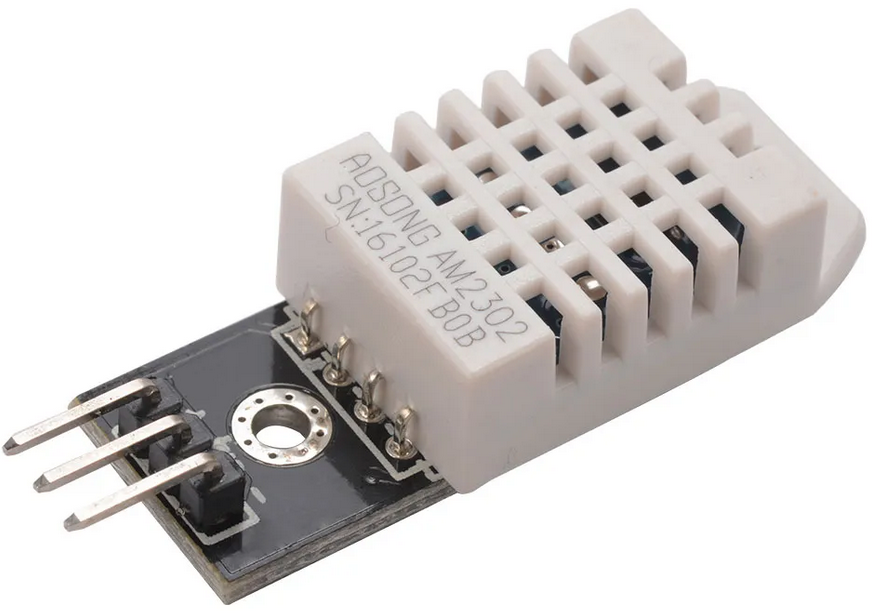
\includegraphics[width=.35\textwidth]{images/sensors/dht22-a.png}\hfill
    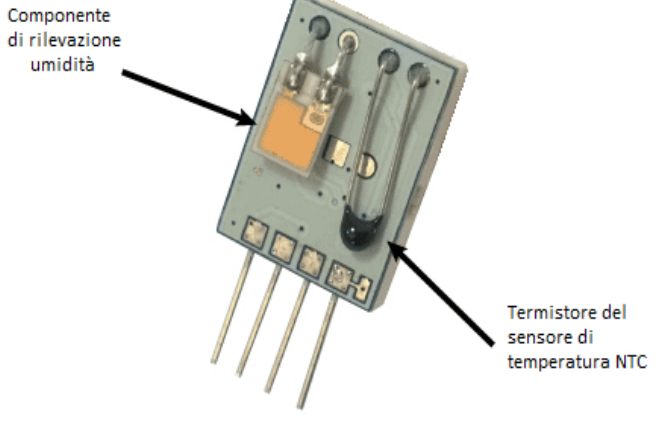
\includegraphics[width=.35\textwidth]{images/sensors/dht22-b.png}\hfill
    \caption{Modulo DHT22.}
\end{figure}

Il dispositivo richiede solamente tre collegamenti con il Raspberry Pi: +5v, terra e un pin GPIO (Tabella \ref*{tb-dht22-conn-schema}).

\begin{table}[H]
    \centering
    \begin{tabular}{|l|l|l|}
    \hline
    \multicolumn{1}{|c|}{\textbf{Modulo PCB}} & \multicolumn{1}{c|}{\textbf{Descrizione}} & \multicolumn{1}{c|}{\textbf{GPIO Pin}} \\ \hline
    GND                                       & Ground                                    & P1-30                                  \\ \hline
    SCL                                       & GPIO 12                                   & P1-32                                  \\ \hline
    VCC                                       & 5V                                        & P1-02                                  \\ \hline
    \end{tabular}
    \caption{\label{tb-dht22-conn-schema}Schema di collegamento modulo DHT22}
\end{table}

\begin{figure}[H]
    \begin{center}
      \includegraphics[width=0.6\textwidth]{images/sensors/DHT22-fritzing.png}
    \end{center}
    \caption{\label{dht22-diagram}Diagramma Fritzing del modulo DHT22.}
\end{figure}

\textbf{ADS1115}\footnote{Link al venditore: \href{shorturl.at/btJVZ}{https://www.amazon.it/AZDelivery-ADS1115}}: convertitore da analogico a digitale, facilmente utilizzabile con una scheda Raspberry Pi utilizzando un bus di comunicazione I2C. Il convertitore ha una buona precisione poiché lavora a 16 bit e sfrutta 4 canali. Le caratteristiche complete del sensore possono essere visionabili alla pagina del \href{https://cdn-shop.adafruit.com/datasheets/ads1115.pdf}{datasheet}. 
Il convertitore utilizza il protocollo di comunicazione I2C per diverse ragioni:
\begin{itemize}
    \item I2C è un protocollo di comunicazione semplice e ampiamente utilizzato, il che lo rende facile da interfacciare con una vasta gamma di microcontrollori e computer singola scheda come Raspberry Pi;
    \item I2C è un protocollo \textit{two-wire}, cioè sono sufficienti solo due fili per il trasferimento dati e la sincronizzazione del \textit{clock}, rendendolo facile da implementare e riducendo il numero di connessioni necessarie;
    \item I2C supporta più dispositivi sullo stesso bus, consentendo a più ADCs di essere collegati allo stesso microcontrollore o computer singola scheda.
\end{itemize}
    
\begin{table}[H]
    \centering
    \begin{tabular}{|l|l|}
    \hline
    \textbf{Caratteristica}   & \textbf{Descrizione} \\ \hline
    Alimentazione             & 2.0$\sim$5.5V        \\ \hline
    Tipo di interfaccia       & I2C                  \\ \hline
    Bit rate ADC              & 16 bit               \\ \hline
    Canali                    & AN0, AN1, AN2, AN3   \\ \hline
    Amplificatore di guadagno & programmabile        \\ \hline
    Dimensioni                & 90 x 52 x 10 mm      \\ \hline
    \end{tabular}
    \caption{\label{ADS1115-features}Caratteristiche principali del modulo ADS1115.}
\end{table}

\begin{figure}[H]
    \centering
    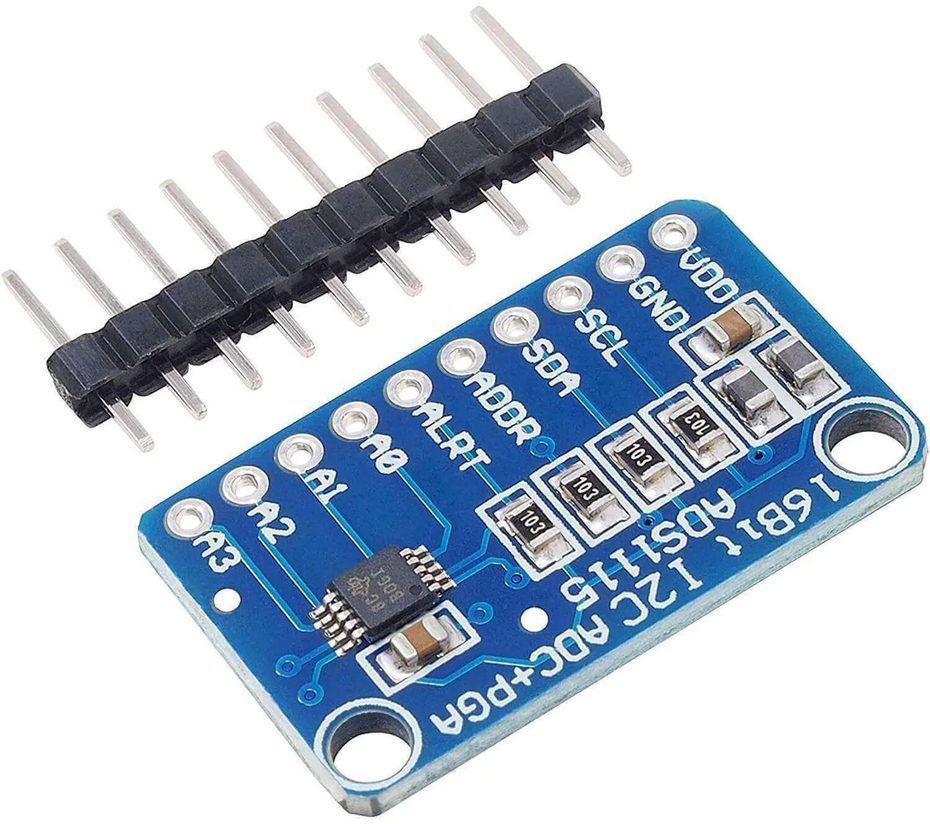
\includegraphics[width=0.35\textwidth]{images/sensors/ads1115.png}\hfill
    \caption{Modulo ADS1115.}
\end{figure}
Il convertitore può essere collegato al Raspberry Pi sfruttando il protocollo I2C (Tabella \ref*{tb-ADS1115-conn-schema}).
\begin{table}[H]
    \centering
    \begin{tabular}{|l|l|l|}
    \hline
    \multicolumn{1}{|c|}{\textbf{Module PCB}} & \multicolumn{1}{c|}{\textbf{Desc}} & \multicolumn{1}{c|}{\textbf{GPIO Header Pins}} \\ \hline
    GND                                       & Ground                             & P1-20                                          \\ \hline
    SDA                                       & I2C SDA                            & P1-03                                          \\ \hline
    SCL                                       & I2C SCL                            & P1-05                                          \\ \hline
    VCC                                       & 3.3V                               & P1-01                                          \\ \hline
    \end{tabular}
    \caption{\label{tb-ADS1115-conn-schema}Schema di collegamento modulo ADS1115.}
\end{table}

\begin{figure}[H]
    \begin{center}
      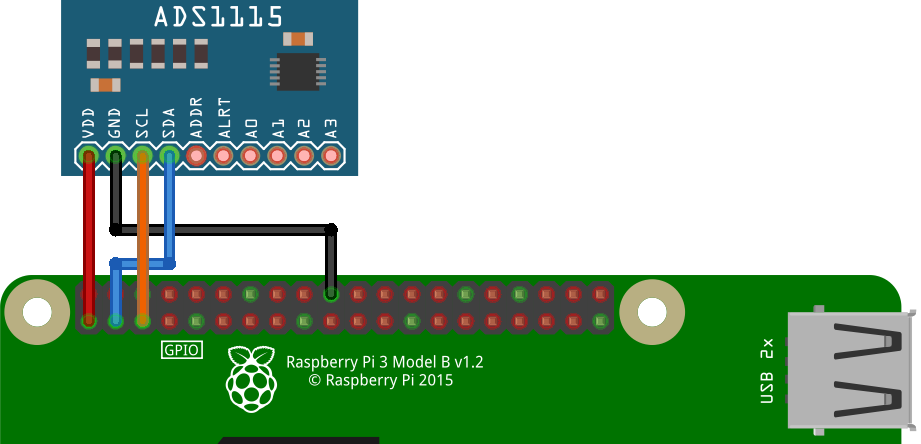
\includegraphics[width=0.6\textwidth]{images/sensors/ads1115-fritzing.png}
    \end{center}
    \caption{\label{ads1115-diagram}Diagramma Fritzing del modulo ADS1115.}
\end{figure}

\textbf{SENSTREE G1/2 CF-B7}\footnote{Link al venditore: \href{https://www.amazon.it/Interruttore-Misuratore-Contatore-Flussometro-Temperatura/dp/B07QNMZ7ZK}{https://www.amazon.it/AZDelivery-CFB7}}: il sensore del flusso d'acqua è costituito da un corpo in rame, un rotore dell'acqua, un magnete e un sensore ad effetto hall. Quando l'acqua scorre attraverso il rotore, questo inizia a girare insieme al magnete. La rotazione del campo magnetico attiva il sensore Hall, il quale emette onde quadre cioè impulsi. Ad ogni giro si avrà un certo volume di acqua che scorre, così come un determinato numero di onde quadre emesse. Pertanto, possiamo calcolare il flusso d'acqua contando il numero di onde quadre.

La formula per il calcolo del flusso d'acqua equivale a:
\[l_{hour} = \frac{flow_{frequency} \cdot 60}{11}\]

Sapendo che, nel caso di CF-B7, il sensore Hall genera 660 impulsi per ogni litro d'acqua, quindi ogni impulso corrisponde a $\frac{1}{660}$ litri. Detto ciò è possibile ricavare il volume totale ($V_{total}(L)$) di liquido che fluisce attraverso il sensore ad un certo tempo $t$, sfruttando il numero di impulsi:
\[V_{total}(L) = N \cdot \frac{1}{660}(L) \]

Inoltre, il volume precedente può essere calcolato anche come $water flow rate(Q - unit L/s)$ moltiplicato per il tempo $t$:
\[V_total(L) = Q(L/s) \cdot t(s) \]

Quindi, si ottiene:
\begin{gather*}
    N \cdot 1/660 = Q(L/s) \cdot t(s) \\
    N/t = 660 \cdot Q(L/s)
\end{gather*}

Infine, siccome $\frac{N}{t}$ equivale alla frequenza $f$:
\begin{gather*}
    f = 660 \cdot Q(L/s) \\
    Q(L/s) = \frac{f}{660} \\
    Q(L/min) = \frac{f \cdot 60}{660} = \frac{f}{11} \\
    Q(L/hour) = \frac{f \cdot 60 \cdot 60}{660} = \frac{f \cdot 60}{11} 
\end{gather*}

\begin{table}[H]
    \centering
    \begin{tabular}{|l|l|}
    \hline
    \textbf{Caratteristica} & \textbf{Descrizione}                \\ \hline
    Alimentazione           & 5$\sim$15 V                         \\ \hline
    Pressione massima acqua & 1,75 MPa                            \\ \hline
    Portata                 & 1$\sim$25L/min                      \\ \hline
    Sensore di temperatura  & NTC 3950 R25 = 50 K.                \\ \hline
    Intervallo di errore    & (1$\sim$30L\textbackslash MIN) ±3\% \\ \hline
    Frequenza               & F=(11*Q) Q=L/MIN ±3\%                 \\ \hline
    Temperatura dell'acqua  & $\leq$ 120°C                              \\ \hline
    Dimensioni              & 65 x 30 x 28 mm                     \\ \hline
    \end{tabular}
    \caption{\label{tb-CF-B7-conn-schema}Caratteristiche principali del modulo CF-B7.}
\end{table}

\begin{figure}[H]
    \centering
    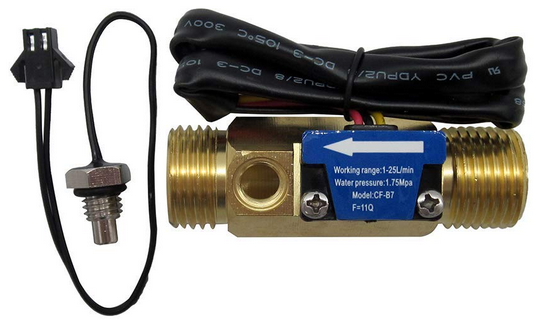
\includegraphics[width=0.35\textwidth]{images/sensors/cfb7.png}\hfill
    \caption{Modulo CF-B7.}
\end{figure}

Come mostrato in Tabella \ref*{tb-CF-B7-conn-schema} il flussometro è provvisto di un foro per l'inserimento di un termistore NTC (Negative Temperature Coefficient) 50K (\href{https://www.tme.eu/Document/34c96454d7432cb275d8954161fb18c2/NTCM-HP-50K-1.pdf}{datasheet}), la cui resistenza elettrica decresce all'aumentare della temperatura. Il sensore ha un ottimo rapporto qualità/prezzo e può essere trovato sul mercato in tante diverse configurazioni.
Per valutare un termistore, la temperatura standard utilizzata dalla maggior parte dei produttori è di 25 °C, che equivale a quella ambiente. Nel caso specifico, a 25° il sensore presenterà una resistenza elettrica di 50K ohm.

Per il calcolo della temperatura ci si affida alla formula semplificata di Steinhart-Hart, cioè alla \textit{B parameter equation}:
%
\[\frac{1}{T} = B \ln{\frac{R}{R_0}} + \frac{1}{T_0}\]
%
Dove $T$ è la temperatura in Kelvin, $R$ è la resistenza del termistore, $R0$ (50K ohm) è la resistenza del termistore a una temperatura nota $T0$ (25 °C) e $B$ è un costante specifica per il termistore (nel caso specifico 3950). 

Il sensore non può essere collegato direttamente al Raspberry perché il segnale deve prima essere convertito da analogico a digitale tramite l'ADS1115. Si è scelto di inserire una resistenza di 10K ohm così da aumentare la risoluzione della misura.
\begin{figure}[H]
    \begin{center}
      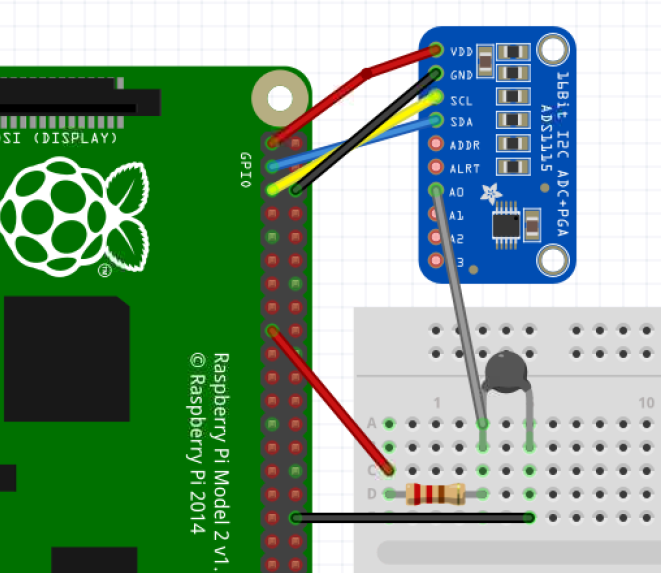
\includegraphics[width=0.6\textwidth]{images/sensors/ntc-fritzing.png}
    \end{center}
    \caption{\label{ntc50k-diagram}Diagramma Fritzing del modulo NTC 50K.}
\end{figure}

\subsubsection{Software}
Come già anticipato le funzionalità della control unit sono state raccolte nei sottodomini Guest Authorization e Room Monitoring. Il primo definisce la gestione del \textit{token} di autorizzazione mentre la seconda descrive la logica di calcolo ed invio dei consumi.
% Dato un discreto numero di concetti di dominio da modellare, ci si è avvalsi del \textit{domain model pattern}. Infatti la business logic viene espressa in termini di:

%     value objects: utilizzati per rappresentare il token di autorizzazione e le varie tipologie di misurazioni (temperatura, corrente, ecc.);
%     entities: sfruttate per definire il concetto di rilevazione (detection) e sensore;
%     domain services: impiegati per modellare la logica di persistenza del token corrente (TokenRepository).

% Il pattern adottato prevederebbe altri elementi costitutivi, come gli aggregators, ma il loro impiego non è stato necessario dato il livello di complessità del dominio.
Inoltre la struttura dell'applicativo è sostenuta da una architettura esagonale (Figura \ref*{clarc}), la quale garantisce caratteristiche quali:
\begin{itemize}
    \item \textit{modularità}: le regole operative possono essere collaudate indipendentemente dalla UI, dal database o qualsiasi altro elemento esterno;
    \item \textit{indipendenza dai framework}: la scelta dei framework ricade solamente sull'ultimo strato dell'architettura, così da utilizzare questi come semplici strumenti evitando di sottostare a specifici vincoli;
    \item \textit{indipendenza dal database}: la business logic non è legata nè a un singolo database nè ad una specifica tipologia.
\end{itemize}

Tutto questo è reso possibile dal rispetto della "regola della dipendenza", la quale sostiene che le dipendenze presenti nel codice sorgente devono puntare solo all'interno, verso le politiche di alto livello. Nella pratica, alcune classi degli strati più esterni vanno ad implementare interfacce definite in quelli più interni. Infatti, la comunicazione con i servizi esterni avviene per mezzo di \textit{adapter} (interfacce) descritti internamente ed opportunamente concretizzati nell'ultimo livello. Inoltre questa tipologia di architettura consente di delineare un confine netto tra i due sottodomini, separando questi in due moduli distinti.
%
\begin{figure}[H]
    \centering
    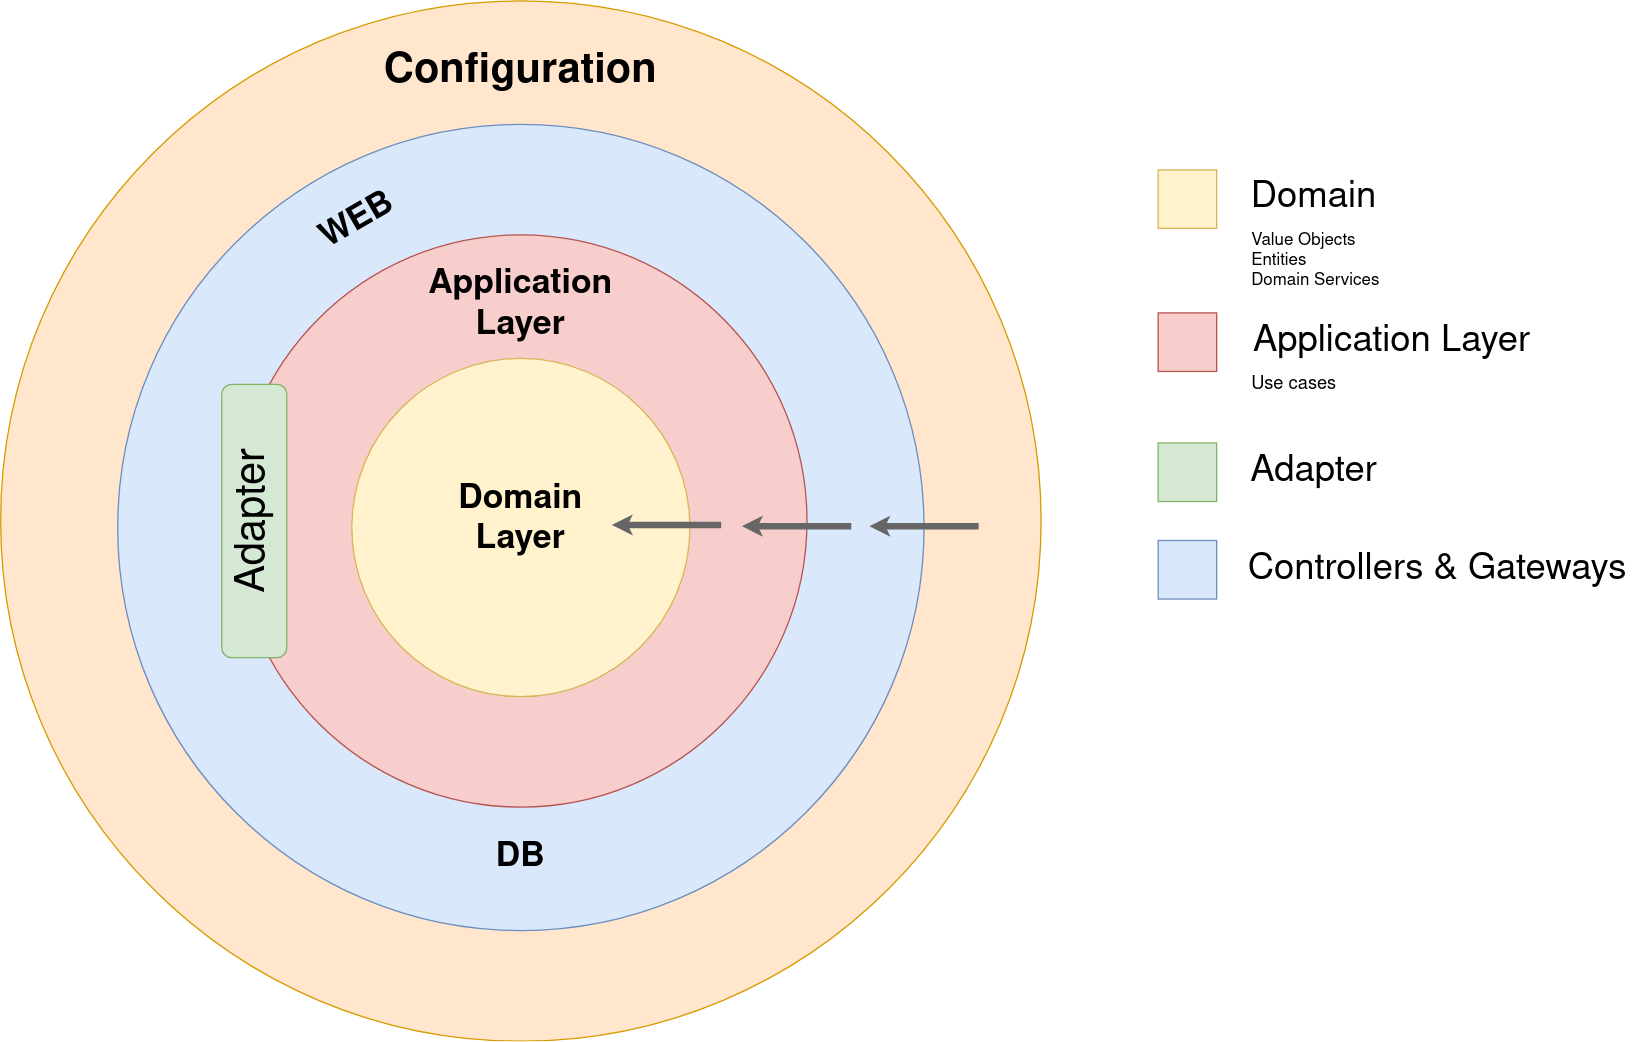
\includegraphics[width=\textwidth]{images/cl-architecture.png}\hfill
    \caption{\label{clarc}Rappresentazione grafica dell'architettura esagonale.}
\end{figure}
%Si può quindi dire che la progettazione della control unit è il risultato della combinazione della terminologia definita dall'ubiquitous language, con gli elementi del domain model pattern ed i concetti dell'architettura esagonale (Figura \ref{cu-uml}).%
Di particolare interesse è la definizione dello strato \textit{core} mediante casi d'uso, questi permettono di orchestrare i flussi di dati da e verso le entità, rimanendo aderenti agli schemi elaborati durante la fase di analisi. In Figura \ref{cu-uml} vengono schematizzati tutti i concetti principali di dominio, alcuni di questi sono semplici contenitori statici di valori (es. \texttt{Resistance}, \texttt{Current}, \texttt{Token}, ecc.) mentre altri definisco la logica dei casi d'uso e necessitano di un rapido approfondimento:
\begin{itemize}
    \item \texttt{EnvironmentUseCases}: racchiude la logica relativa al rilevamento dei fattori ambientali tramite i sensori di flusso dell'acqua, luminosità, temperatura e umidità;
    \item \texttt{ConsumptionUseCases}: come si evince dal nome, si occupa della raccolta dei consumi idrici ed elettrici;
    \item \texttt{AuthorizationUseCases}: set di funzionalità fondamentali per l'avvio della centralia, la ricezione/comunicazione del \textit{token} d'accesso e l'implementazione del protocollo di comunicazione tra la \textit{control unit} e uno smartphone nelle vicinanze.
\end{itemize}
\begin{figure}[H]
    \centering
    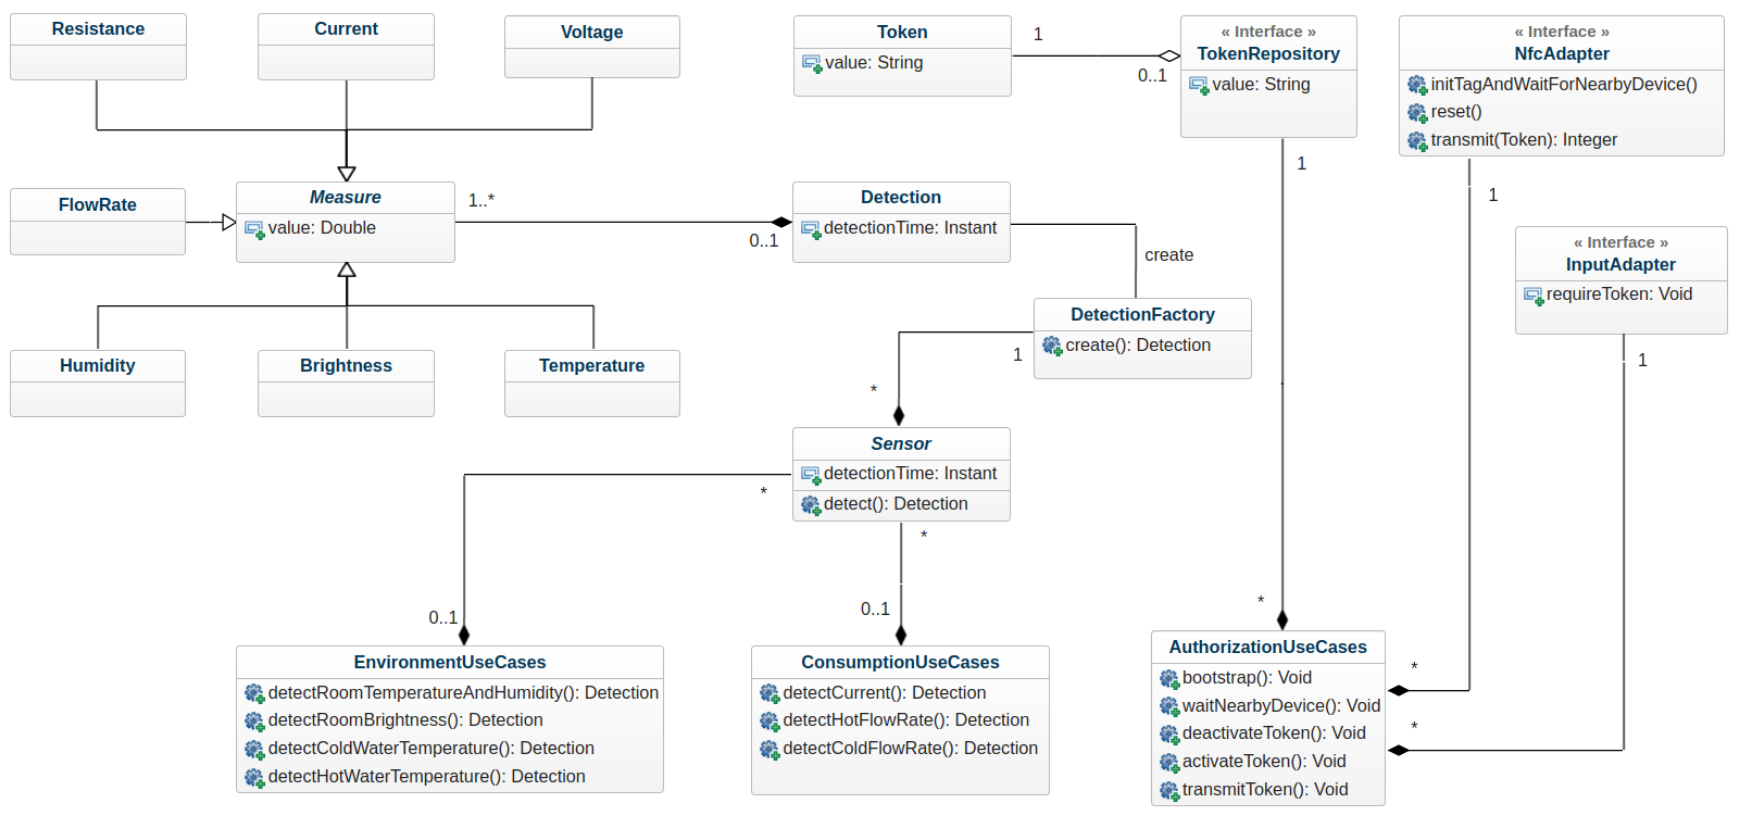
\includegraphics[width=\textwidth]{images/cu-uml.png}\hfill
    \caption{\label{cu-uml}Modellazione dei concetti di dominio tramite UML delle classi.}
\end{figure}
Nel caso delle rilevazioni, i dati prodotti vengono assegnati ad una specifica istanza di \texttt{Detection} che, oltre includere il valore rilevato, è associata alla data di creazione e ad un \textit{id} che la identifica univocamente. 
%
\begin{figure}[H]
    \centering
    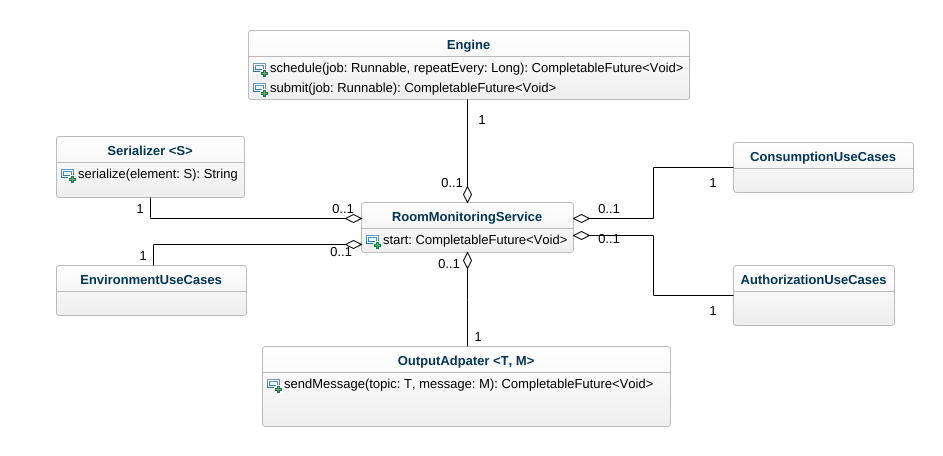
\includegraphics[width=\textwidth]{images/room-monitoring-serivce.png}\hfill
    \caption{\label{rm-uml}Diagramma UML delle classi (\texttt{RoomMonitoringService}).}
\end{figure}
%
Infine la logica di monitoraggio della stanza (\textit{Room Monitoring}) è racchiusa all'interno della classe \texttt{RoomMonitoringService} (Figura \ref*{rm-uml}). Questa, tramite un proprio flusso di controllo, esegue periodicamente (ogni 5 secondi) ed in maniera concorrente tutti i rilevamenti necessari (consumi e ambiente), interrompendoli nel caso di superamento del \textit{timeout}. Una volta ottenuti tutti i risultati, questi vengono prima serializzati grazie un'istanza di \texttt{Serializer} e successivamente comunicati verso l'esterno tramite l'\texttt{OutputAdapter}. Data la natura concorrente del servizio, si è scelto di schematizzarne il comportamento attraverso un diagramma di stato (Figura \ref*{rm-uml-state}).

\begin{figure}[H]
    \centering
    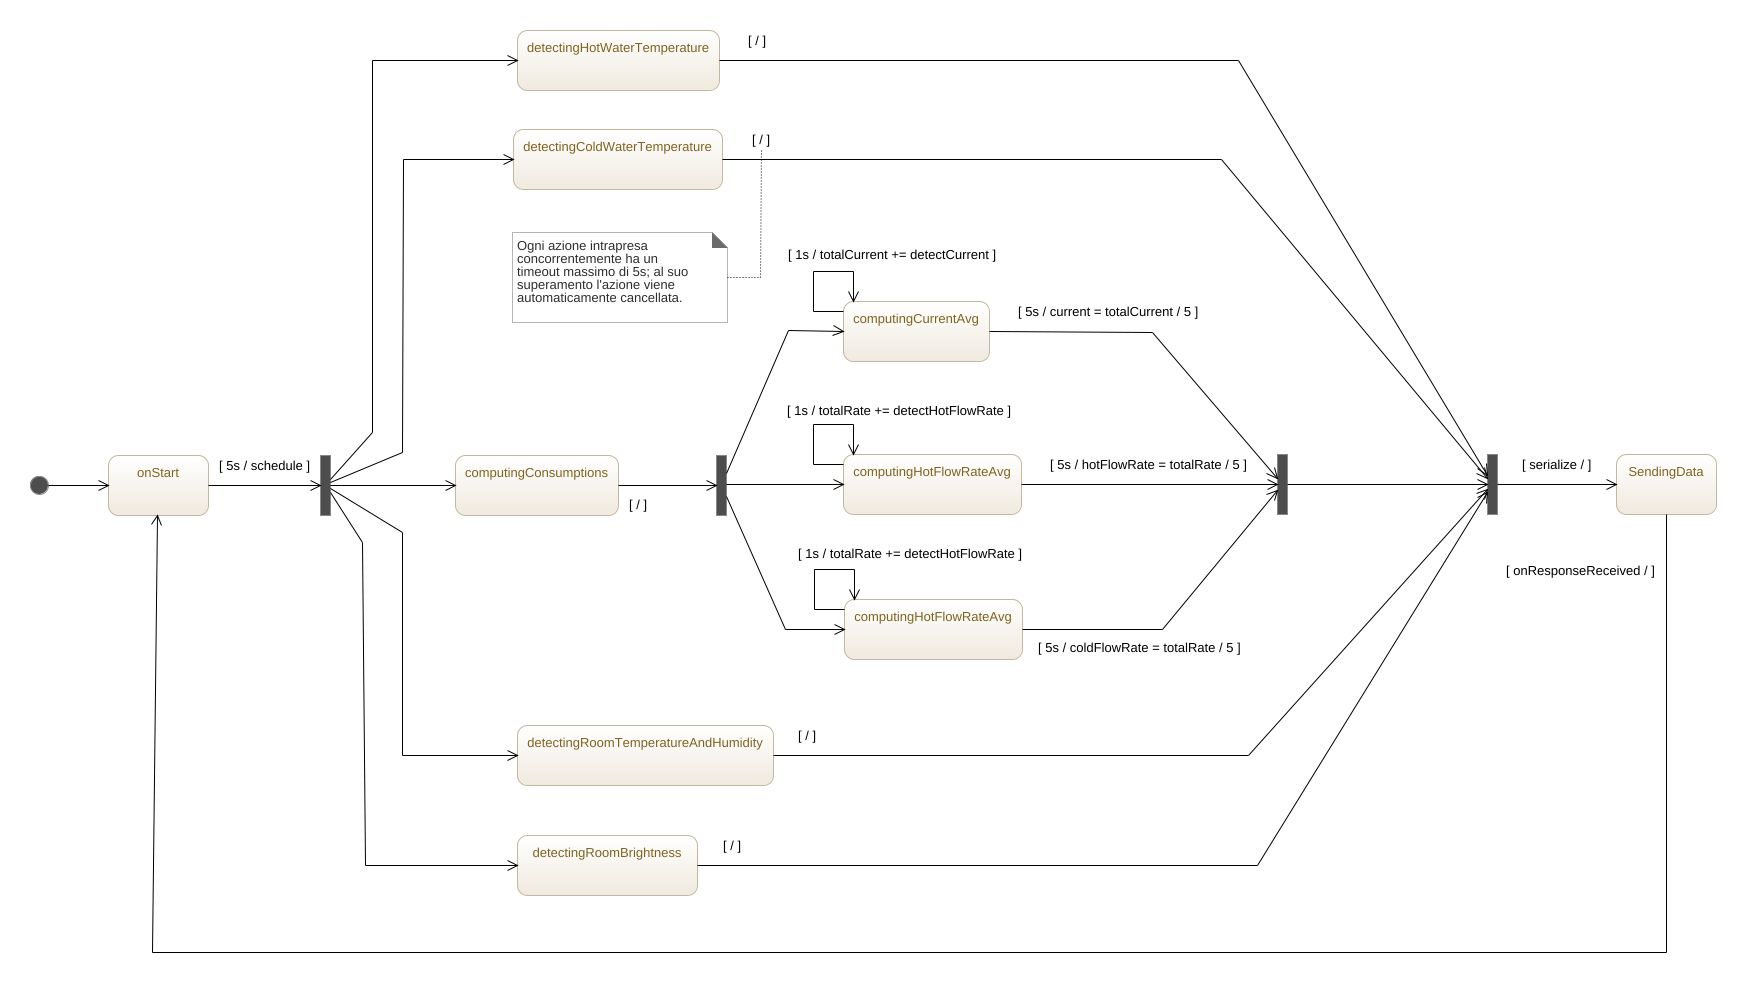
\includegraphics[width=\textwidth]{images/room-monitoring-service-state-diagram.jpeg}\hfill
    \caption{\label{rm-uml-state}Diagramma UML di stato (\texttt{RoomMonitoringService}).}
\end{figure}

\subsection{Administration}
\begin{itemize}
    \item Descrivere come funziona l'Administration e il pannello di controllo cone le eventuali rotte REST
    \item Diagramma ER (Room, Hotel, Stay ecc.)
\end{itemize}


\newpage
%----------------------------------------------------------------------------------------
%	IMPLEMENTAZIONE
%----------------------------------------------------------------------------------------

\section{Implementazione}\label{sec:implementazione}
Similmente a quanto fatto nella sezione precedente, anche in questo caso le soluzioni implementative avanzate sono state suddivise per sottodomonio. Di ognuna si elencano le motivazioni e le problematiche emerse durante lo sviluppo. 

\subsection{Control Unit}
Per quanto riguarda la centralina, prima di avviare il vero e proprio sviluppo del progetto si è scelto di verificare il corretto funzionamento dei sensori, collegando ciascuno di essi alla scheda e validando l'output restituito tramite opportuni software rilasciati dal produttore. Nello specifico, siccome diversi sensori comunicano mediante protocollo I2C, è stato necessario collegare questi a una \textit{breadboard} al fine di ampliare il numero di ingressi disponibili ai GPIO SDA e SCL. Una volta completata la fase preliminare di sperimentazione si è passati alla realizzazione di una \textit{build multi-progetto} confinando le funzionalità all'interno di moduli indipendenti, al fine di semplificare l'attività di sviluppo parallela tra i membri del team. Come già anticipato nella sezione di progettazione, il progetto si compone di diversi strati, quelli più interni realizzano la logica di \textit{business} che deve essere totalmente indipendente da \textit{framework}. I livelli più esterni invece dipendo dalla libreria \href{https://pi4j.com/}{Pi4J} (versione 2), la motivazione principale è stata la ricerca di un livello di astrazione che potesse nascondere gli aspetti di basso livello, permettendo così al team di concentrasi quasi esclusivamente sulla logica di \textit{business}. Ovviamente vi sono altri vantaggi derivanti dall'adozione di Pi4J e possono essere riassunti in:
\begin{itemize}
    \item \underline{Facilità d'uso}: Pi4J espone un'API semplice e intuitiva in Java che facilita l'interazione con la componente hardware, cioè con i pin GPIO del Raspberry;
    \item \underline{Supporto per più periferiche}: Pi4J supporta anche altri dispositivi periferici connessi al Raspberry Pi come dispositivi I2C e SPI;
    \item \underline{Manutenzione}: Pi4J è attivamente mantenuta da una comunità di sviluppatori, questo comporta la risoluzione di eventuali bug ed estensioni future;
    \item \underline{Grande comunità}: in rete vi sono numerose risorse (es. classi Java che modellano il comportamento di specifici sensori) e un ampio supporto per la risoluzione dei problemi;
    \item \underline{Open-source}.
\end{itemize}
Il \textit{framework} Pi4J, da una parte ha agevolato lo sviluppo architetturale ma dall'altra ha reso gli \textit{script} forniti dai produttori inutilizzabili, vincolando quindi il team a riscrivere le logiche dei singoli sensori. Le classi prodotte sono quindi il risultato di una ricerca basata sugli \textit{script} dei fornitori, i \textit{datasheet} dei sensori e le risorse in rete messe a disposizione dalla \textit{community}.
\newline\newline
Siccome il software della centralina si compone di due servizi, cioè \textit{Authorization} e \textit{RoomMonitoring}, fin da subito si è optato per l'adozione del paradigma concorrente così da eseguire i due servizi in flussi di controllo separati. Nella pratica si è realizzata una classe \texttt{Engine} che aggiunge un livello di astrazione rispetto allo \texttt{ScheduledExecutorService} della libreria \texttt{java.util.concurrent}. Concretamente i servizi vengono lanciati nel seguente modo:
\lstinputlisting[caption={Setup e avvio dei servizi.}, label={lst:main}, language=Java]{code/main.java}
%
Come mostrato nel Listato \ref{lst:main}, per ogni servizio viene istanziato un \texttt{Engine} fatta eccezione per l'\texttt{awsAdapter} che, appoggiandosi sulla libreria \texttt{software.amazon.awssdk}, già esegue all'interno di un flusso di controllo indipendente.L'\texttt{awsAdapter} si occupa di inoltrare i dati prodotti dal \texttt{RoomMonitoringService} verso il \textit{backend} tramite protocollo MQTT e realizza lo \textit{shadowing} tra la centralina e la sua copia digitale. 
Inoltre l'\texttt{awsAdapter} registra l'\texttt{AuthorizationService} come "osservatore" così da notificargli eventuali modifiche del \textit{token} di accesso. Infine, l'avvio dei servizi avviene solamente conclusa la procedura di \textit{bootstrap}, cioè di connessione con il \textit{backend}.
%
\subsubsection{RoomMonitoringService}
Internamente il \texttt{RoomMonitoringService} (Listato \ref*{lst:rms}) esegue ogni $N$ secondi il calcolo dei consumi (corrente e acqua divisa in calda e fredda) e rileva i fattori ambientali della stanza (temperatura, umidità, luminosità). I dati raccolti vengono prima serializzati e poi inviati verso l'esterno. I consumi vengono calcolati più volte durante gli $N$ secondi, infatti è prevista una logica di aggregazione. Tutte le funzionalità implementante sono asincrone poiché si avvalgono delle \texttt{CompletableFuture} di Java.
\lstinputlisting[caption={Logica \textit{core} del \texttt{RoomMonitoringService}.}, label={lst:rms}, language=Java]{code/RoomMonitoringService.java}
%
\subsubsection{AuthorizationService}
L'\texttt{AuthorizationService} esegue solo un \textit{task} bloccante definito in due step: \texttt{bootstrap()} e \texttt{startNfcTagEmulation()}. Il primo provvede a sincronizzare lo stato della centralina con quello memorizzato sul \textit{backend}, mentre il secondo abilita la connessione tra lo smartphone e il lettore NFC. Come mostrato nel Listato \ref*{lst:as}, la funzione \texttt{startNfcTagEmulation} viene ripetuta anche nel caso di due errori specifici. Quest'ultimi non sono considerati fatali poiché possono essere provocati, per esempio da un allontamento precoce dello smartphone dal lettore.
\lstinputlisting[caption={Logica \textit{core} dell'\texttt{AuthorizationService}.}, label={lst:as}, language=Java]{code/AuthorizationService.java}
%
Il codice del programma che permette di convertire i dati ottenuti dal sensore BH1750 in \texttt{lux} (Listato \ref*{lst:bh}), si avvale della classe \texttt{I2C} di Pi4j che, grazie al metodo \texttt{read}, restituisce i due byte (LSB e MSB) necessari per produrre il risultato.
\lstinputlisting[caption={Progammazione del modulo BH1750.}, label={lst:bh}, language=Java]{code/BH1750.java}
%
\subsubsection{DHT22}
Nel caso del modulo DHT22, la programmazione del sensore ha richiesto uno sforzo maggiore poiché si è riscontrata una problematica legata all'interfaccia \texttt{Digital} fornita dalla libreria Pi4J. Questa permette di comunicare con un pin GPIO del Raspberry mediante due classi: \texttt{DigitalOutput} e \texttt{DigitalInput}. Quindi non è possibile creare un collegamento sul quale scrivere e leggere contemporaneamente. Questo si è rivelato una limitazione perché il protocollo del DHT22 richiede nello stesso ciclo di polling, una comunicazione sia in input che in output, ma il tempo richiesto per la riconfigurazione del pin provoca un ritardo che quasi sempre supera la finestra di 40-80 microsecondi richiesta dal protocollo. Ciò comporta una perdita di informazioni che può provocare errori nella trasmissione. Si è quindi scelto di realizzare un \textit{fork} di Pi4J al fine di aggiungere le funzionalità richieste all'interno di una nuova classe chiamata \texttt{DigitalMultiPurpose}. Questa implementazione permette di interagire con un pin in entrambe le modalità riducendo i tempi allo scopo di rientrare all'interno della finestra temporale prima citata. Della libreria Pi4J è stato modificato anche il file di \textit{build} di \textit{Maven} così da permettere la pubblicazione degli artefatti (\textit{package}) all'interno di Github Packages automatizzandone il download tramite Gradle.
%
\subsubsection{Flussometro}
Per quanto riguarda il flussometro, è stato sufficiente utilizzare un istanza di \texttt{DigitalInput} messe a disposizione da Pi4J. A questa è stata associata una \textit{callback} che si occupa di incrementare un contatore ogni qualvolta il pin si trovi nello stato di \texttt{HIGH}. Dopo un secondo (circa) il contatore degli impulsi viene suddiviso per la frequenza specifica del sensore così da ottenere i litri di acqua fluiti (L/s). Al fine di ottenere un risultato più accurato, si tiene traccia del tempo effettivamente trascorso da una rilevazione e l'altra.
\lstinputlisting[caption={Progammazione del flussometro.}, label={lst:wfs}, language=Java]{code/WaterFlowSensor.java}
%
\subsubsection{NTC - Termistore}
Come già anticipato nella sezione progettuale, per il calcolo della temperatura tramite termistore ci si affida ad una versione semplificata dell'equazione di Steinhart-Hart. L'utilizzo della costante \texttt{KELVIN} (273.15) permette di convertire il risultato ottenuto in Celsius. Poiché il termistore utilizzato è un dispositivo analogico, il parametro \texttt{inputVoltage} viene fornito dall'ADC a sua volta astratto mediante una specifica classe Java.
\lstinputlisting[caption={Progammazione del termistore NTC 50K.}, label={lst:ntc}, language=Java]{code/NTCSensor.java}
% 
\subsubsection{PN532}

Il modulo NFC nel nostro caso non si occupa di leggere TAG, ma di stabilire una comunicazione con uno smartphone al fine di inviargli il token.
Più precisamente si è riusciti ad eseguire questa operazione senza un app nativa sul dispositvo cellulare: 
è infatti sufficiente avvicinare lo smartphone al controller NFC perchè questo si attivi ed invii URL con il token lanciando la web app sul dispositivo.

Per fare questo il controller NFC viene inizalizzato via software nella modalità "card emulation", il PN532 è quindi capace di rispondere a comandi "Reader/Writer" 
secondo lo schema standard ISO/IEC 14443A/MIFARE.

Nell'implementare questa modalità di comunicazione si sono seguite le specifiche di "NFC Forum Type 4 Tag".
Un Tag Type 4 contiene un messaggio NFC Data Exchange Format (NDEF) il quale include il nostro URL con il token.

Il controller PN532 ci ha dato dapprima problemi di stabilità di connessione con l'interfaccia I2C, che ci ha costretti a connetterlo al canale SPI.
In secondo luogo abbiamo dovuto riportare tutto il protocollo di comunicazione in linguaggio Java e questo ha richiesto una gran quantità di debugging.

Attualmente il controller funziona solo comunicando con dispositivo modello iPhone, occorre più tempo per supportare altri device e rendere tutto più stabile. 

\newpage
%----------------------------------------------------------------------------------------
%	ANALISI DI DEPLOYMENT SU LARGA SCALA
%----------------------------------------------------------------------------------------

\section{Analisi di deployment su larga scala}
Il paradigma a microservizi da noi adottato si adatta perfettamente al deployment su larga scala.
Il progetto è stato fin da subito pensato per l'esecuzione in cloud, utilizzando appieno gli Amazon Web Services anche durante lo sviluppo locale.

Di seguito descriveremo in prima fase l'architettura adottata per il deployment, 
passeremo poi ad illustrare come viene praticamente eseguito il deployment sui vari ambienti (locale, staging e production), 
ed infine quali sono i costi totali del sistema. 

\subsection{Architettura Cloud}

Il progetto Ecotrip si basa sul raccogliere dati da una moltitudine di camere di una moltitudine di hotel, 
analizzarli ed aggregarli al fine di calcolare punteggi da fornire ad una moltitudine di utenti (visitatori e albergatori).

In prima battuta però Ecotrip verrà adottato da un singolo Hotel, è chiara quindi l'esigenza di un'architettura di deployment 
che consenta di partire con costi ridotti e che permetta una scalabilità orizzontale al bisogno.

Per ottenere questo abbiamo impiegato il paradigma Serverless per le componenti che richiedono una forte scalabilità, 
come il caricamento e lo stoccaggio dei dati, l'elaborazione e la fornitura verso gli utenti finali. 
Serverless significa impiegare servizi Cloud che scalano in automatico all'occorrenza, senza alcuna pianificazione prestabilita o intervento umano.

In Figura 22 mostriamo l'architettura implementata utilizzando diversi servizi messi a disposizione da Amazon Web Services (AWS).

Poiché questo è un progetto IoT, abbiamo scelto di utilizzare \textbf{DynamoDB}, il database serverless fornito da AWS, il quale è in grado di scalare automaticamente sia per quello che concerne la quantità di dati che per il numero di richieste al secondo.
Abbiamo suddiviso il database in tre tabelle: "IoTData" per i dati IoT inviati dalla Control Unit, "Administration" per la gestione della REST API, e "DataElaboration" per l'elaborazione dei dati. 
Questa suddivisione ci permette di gestire in modo efficiente e organizzato i dati del progetto, strutturando al meglio ogni tabella secondo le logiche di data modelling per un database NoSQL di tipo Key-Value.
Da notare che le entità di \textit{Administration} illustrate in fase progettuale sono confluite nella pratica in un'unica tabella DynamoDB: per arrivare a questo risultato abbiamo seguito le best-practices per il design di database NoSQL che richiede un approccio diverso dalla progettazione di RDBMS.

\begin{figure}[H]
    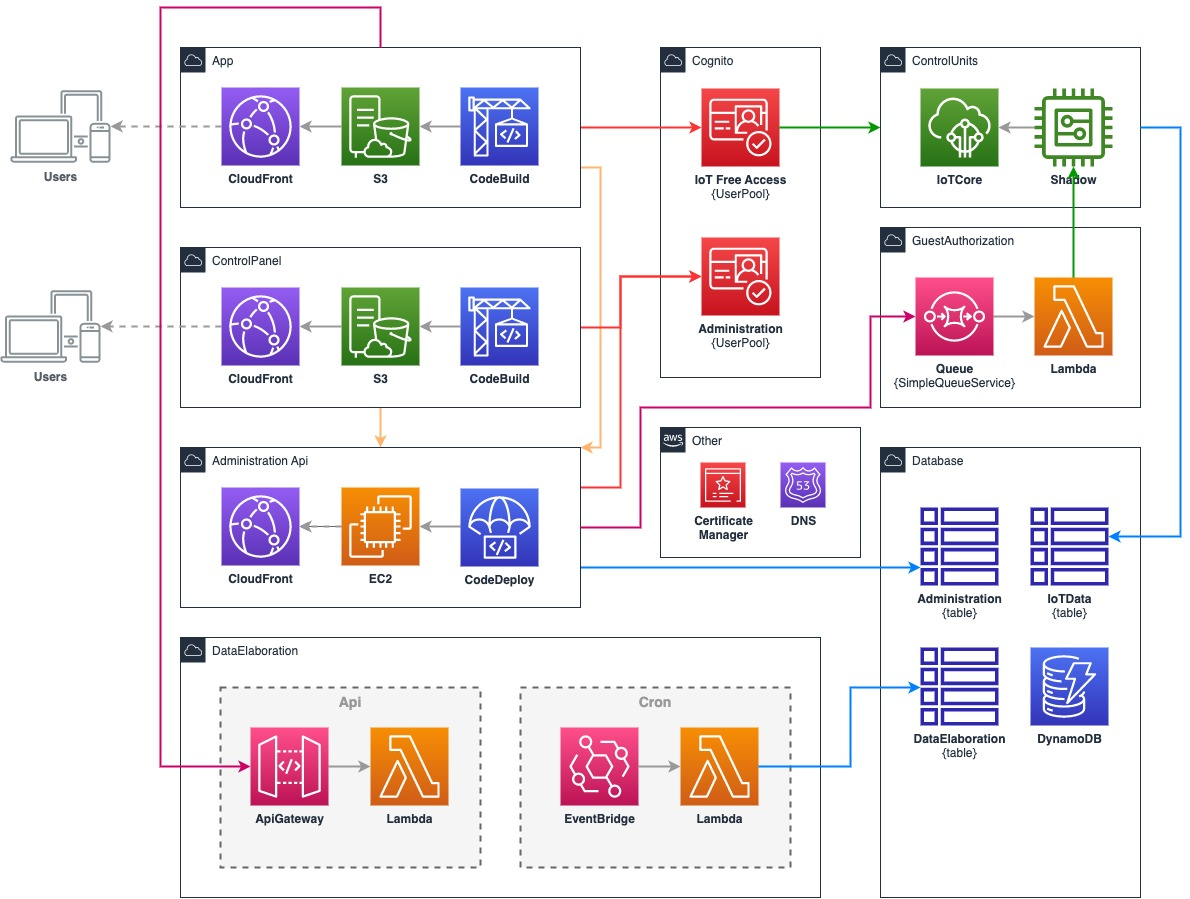
\includegraphics[width=\textwidth]{AWS.jpg}
    \centering
    \caption[aws]{Architettura AWS}
    \label{fig:aws}
\end{figure}

Il servizio \textbf{IoT Core} gestisce le centraline IoT e il loro stato attraverso la \textbf{copia shadow}. La copia shadow rappresenta una versione virtuale dello stato di ogni centralina IoT, che viene mantenuta sincronizzata con la centralina stessa. Inoltre si preoccupa di ricevere i dati delle centraline attraverso messaggi MQTT e stoccarli attraverso una opportuna regola sulla tabella IoTData.

La \textbf{REST API} della parte "Administration" è distribuita attraverso una istanza \textbf{EC2}.
Il traffico richiesto per questo componente è relativamente basso in quanto la API "Administration" è soprattutto utilizzata dal pannello di controllo, e si assume che vengano fatte richieste contemporanee da al massimo un utente per hotel, oltre ai visitatori che attraverso le app ricevono limitate informazioni sull'hotel (il nome) e il pernottamento corrente.
Per questo, in questa prima fase, si è scelto di non dotare il servizio API di scaling automatico tramite l'aggiunta di un load balancer.
In futuro la EC2 potrebbe essere sostituire da un servizio API Gateway che consente la completa scalabilità on demand tramite l'impiego di Lambda per ogni endpoint.

Le applicazioni single page (SPA) del pannello di controllo e web app sono distribuite tramite \textbf{CloudFront} di Amazon Web Services ed archiviate in un bucket S3. CloudFront è una rete di distribuzione dei contenuti (CDN) su server dislocati in tutto il mondo, il che garantisce una bassa latenza e una consegna veloce per gli utenti, indipendentemente dalla loro posizione geografica.

La generazione del token per i visitatori del microservizio "Guest Authorization" avviene su una \textbf{Lambda}, questa si attiva alla ricezione di un messaggio inviato da "Administration" attraverso il servizio di coda \textbf{Simple Queue Service} impostato in modalità FIFO (FirstIn-FirstOut). La Lambda si occuperà di aggiornare il valore del token sulla copia shadow del dispositivo fisico, dopo averlo ricercato all'interno del servizio IoT Core attraverso attributi univoci che identificano la centralina di una determinata stanza di un albergo.

Per l'elaborazione dei dati da parte di "Data Elaboration" è stata impiegata un'altra Lambda che si attiva periodicamente ogni 5 minuti attraverso un'attività pianificata di tipo \textbf{EventBridge}. Dopo aver eseguito i calcoli questi vengono memorizzati su un apposta tabella "DataElaboration" in DynamoDB.
Attualmente i dati da elaborare vengono processati da un unica istanza della Lambda, ma è possibile strutturare il sistema in modo che ogni hotel avvii la sua istanza di Lambda periodicamente per processare unicamente i suoi dati: questo consente la totale scalabilità computazionale anche per quanto riguarda questo servizio che è il più critico ed oneroso in termini di costo di CPU.
La fornitura dei dati elaborati, come i consumi di un pernottamento o il punteggio sostenibilità richiesti dai visitatori o albergatori, avviene attraverso una REST API realizzata con \textbf{API Gateway}: servizio di Amazon che permette ad una API di abbracciare in pieno il paradigma Serverless e quindi piena scalabilità on-demand.

Per quanto riguarda la gestione degli utenti, abbiamo utilizzato \textbf{Cognito}. Abbiamo creato due diverse pool di utenti: una per il pannello di controllo "Administration" e un'altra per gli accessi liberi "IoT Free Access". La pool di utenti "Administration" fornisce l'accesso al pannello di controllo per gestire la configurazione e gestione degli alberghi, stanze e prenotazioni. La pool di utenti "IoT Free Access", d'altra parte, consente agli utenti sull'App di visualizzare i dati MQTT in tempo reale della parte IoT senza la necessità di una registrazione.
Cognito emette un token di autorizzazione per ogni sessione di accesso degli utenti, che può essere utilizzato per autorizzare le richieste API. Il token di autorizzazione scade dopo un certo periodo di tempo, ma gli utenti possono ottenere un nuovo token di autorizzazione tramite il token di refresh. Questo sistema a due token garantisce la sicurezza dei dati degli utenti e delle applicazioni, poiché i token di autorizzazione possono essere revocati o scadere in qualsiasi momento, senza che ciò influisca sulla sessione di accesso degli utenti. 

\subsection{Ambienti di deployment}

Il deployment è un aspetto cruciale per questo tipo di progetto, per questo ci siamo concentrati subito sul definire come lavorare e sviluppare in locale con i servizi cloud.

Abbiamo predisposto 3 ambienti: \textbf{locale}, \textbf{staging} e \textbf{production}.

Per quanto riguarda lo sviluppo in locale, abbiamo creato un ambiente che riproduce l'architettura descritta in precedenza. 
Utilizzando \textbf{Docker Compose}, abbiamo emulato le due Applicazioni (App e ControlPanel), la REST API e il database DynamoDB in container separati. Mentre per quanto riguarda i servizi rimanenti (Cognito, DataElaboration e GuestAutorizzazione) abbiamo utilizzato script che compilano ed avviano template in \textbf{SAM} per creare stack in \textbf{CloudFormation}, effettuando così il deploy direttamente su AWS dei servizi per il singolo componente del team. 
In questo modo il team di sviluppo può lavorare sul progetto in modo semplice e rapido. Tutto ciò che serve è scaricare il repository che include tutti i sotto-moduli necessari. Con un semplice script, l'ambiente locale viene preparato utilizzando Docker Compose e la parte online su AWS viene avviata attraverso stack di CloudFormation. Questo processo viene effettuato in modo specifico per ogni singolo membro del team, garantendo così un ambiente di sviluppo personalizzato e indipendente.

SAM (\textbf{Serverless Application Model}) è un framework opensource che attraverso modelli permette di descrivere l'architettura cloud da creare e gestire. SAM è stato progettato per semplificare la creazione e la gestione di applicazioni serverless utilizzando CloudFormation, senza dover accedere manualmente alle interfacce di gestione di AWS.

In fase di staging e production, il processo di deployment viene completamente automatizzato tramite le \textbf{GitHub Action} sulle apposite branch. Queste azioni avviano i relativi script che attraverso i template SAM creano e mantengono aggiornata l'infrastruttura su AWS, garantendo così un processo di distribuzione affidabile, efficiente e privo di errori. Il sistema di deploy automatico garantisce che il progetto sia sempre allineato alla versione più recente.

L'ambiente di staging è una replica fedele dell'ambiente di produzione, che viene utilizzato per effettuare test e verifiche prima di effettuare eventuali modifiche al sistema in produzione. Questo ambiente separato permette di effettuare prove senza influire sul funzionamento e sui dati del sistema in produzione, garantendo così la stabilità e la sicurezza dell'intero ecosistema.

\newpage

%----------------------------------------------------------------------------------------
%	TESTING E PERFORMANCE
%----------------------------------------------------------------------------------------

\section{Testing e performance}

Lo sviluppo del progetto è progredito con metodologia incrementale e con test automatizzati per tutte le sue parti critiche. 
Ogni componente è quindi adeguatamente testato singolarmente nelle sue logiche di funzionamento.

A prototipo concluso si sono eseguiti manualmente test integrativi andando a verificare l'effettivo funzionamento del sistema nel suo insieme.
A tal fine, sono stati eseguiti i seguenti passi:
\begin{itemize}
    \item deployment dei diversi servizi web in abiente \textit{production}
    \item accesso al pannello di controllo con l'utente super amministratore pre configurato
    \item aggiunto da pannello di controllo un hotel di prova con il rispettivo account per l'albergatore
    \item aggiunta da pannello di controllo una camera all'hotel
    \item avviata la centralina
    \item installata e configurata da pannello IoT Core specificando hotel e camera come suoi attributi
    \item verificata la ricezione dei dati 
    \item verificata la correttezza dei dati in base alle sollecitazioni dei vari sensori
    \item eseguito da pannello di controllo un check-in per la camera generando il token
    \item verificato il calcolo del punteggio sostenibilità per il pernottamento di prova
    \item avviata la web app avvicinando lo smartphone al controller NFC
\end{itemize}

Non si sono riscontrati problemi tranne per l'invio del token al dispositivo cellulare mediante NFC: 
permane un problema che riguarda l'inizializzazione del controller NFC che a volte non avviene con successo. 
Abbiamo trovato un work-around ma il fix del problema richiede una sessione di debugging approfondita che riguarda 
il protocollo "NFC Forum Type 4 Tag".

Riguardo le performance del sistema, è possibile discutere di due componenti critiche: \textit{Control Unit} e \textit{Data Elaboration}.

Per la centralina si segnala che, per quanto l'implementazione in Java sia del tutto inefficiente e ci ha costretti ad eseguire campionamenti ripetuti su diversi sensori in modalità polling, 
l'utilizzo della CPU del Raspberry PI4 non supera il 12\% con una media intorno al 8\%.
Questo significa che, adottando anche un implementazione in C, possiamo ridurre di molto le caratteristiche dell'hardware e quindi risparmiare sui costi finali del prodotto.
Per quello che concerne l'invio dei dati con il protocollo MQTT, poichè questo avviene ogni 5 secondi ed il messaggio è di dimensione molto ridotta, non vi sono particolari analisi di performance da effettuare.

Per il componente \textit{Data Elaboration} la cui AWS Lambda si attiva periodicamente ogni 5 minuti abbiamo rilevato un tempo di esecuzione medio di 900 ms con utilizzo di RAM medio pari a 120 MB:
qui sono sicuramente possibili degli interventi volti a migliorarne le performance e ridurre i costi di servizio.

\newpage
%----------------------------------------------------------------------------------------
%	PIANO DI LAVORO
%----------------------------------------------------------------------------------------

\section{Piano di lavoro}

Lo sviluppo del progetto Ecotrip ha coinvolto il team per uno span temporale relativamente lungo di circa 8 mesi, 
in quanto è stato inserito in mezzo a impegni di lavoro.
Indicativamente ogni componente del team ha svolto più di 1 mese e mezzo di attività di sviluppo per giungere al prototipo finale, 
questo è andato oltre le aspettative iniziali ma con la consapevolezza che l'impegno potrebbe portare ad una startup 
con il nostro partner commerciale.

La prima fase del progetto è stata svolta dall'intero team per circa 1 settimana nel mese di Giugno 2022, ed ha compreso:
\begin{itemize}
    \item ideazione e knowledge crunching con il partner
    \item studio preliminare di fattibilità
    \item progettazione strategica e architetturale
    \item stesura dei requisiti
    \item impostazione e creazione dei repo di lavoro
\end{itemize}

Si è poi proceduto con lo sviluppare singoli sezioni del progetto, da qui ogni componente del team ha lavorato singolarmente o al massimo in coppia.

Di seguito illustreremo per ogni componente del team ciò che è stato fatto in ordine cronologico.

Alan Mancini
\begin{itemize}
    \item Control Unit: ricerca, selezione e acquisizione dei sensori (2gg - Giugno 2022)
    \item Control Unit: studio ed integrazione framework PI4J (2gg - Giugno 2022) 
    \item Control Unit: installazione e sperimentazione dei vari sensori (7gg - Giugno 2022)
    \item Control Unit: implementazione architettura esagonale e logica applicativo (7gg - Settembre 2022)
    \item Control Unit: fork e miglioramenti a PI4J (7gg - Novembre 2022)
    \item Control Unit: programmazione sensore ACS712 (2gg - Novembre 2022)
    \item IoT Core: studio DynamoDB (1gg - Novembre 2022)
    \item IoT Core: studio e configurazione regole storicizzazione (1gg - Novembre 2022)
    \item Control Unit: studio AWS IoT Device per stato shadow (1gg - Dicembre 2022)
    \item Control Unit: programmazione NFC PN532 (8gg - Dicembre 2022)
    \item Guest Authorization: studio AWS Lambda con SQS e implementazione (5gg - Gennaio 2023)
\end{itemize}

Alberto Marfoglia
\begin{itemize}
    \item Control Unit: impostazione progetto Gradle e Continuous Integration (2gg - Giugno 2022) 
    \item Control Unit: ricerca framework per Raspberry (1gg - Giugno 2022) 
    \item Control Unit: installazione e sperimentazione dei vari sensori (7gg - Giugno 2022)
    \item Control Unit: implementazione architettura esagonale e logica applicativo (14gg - Settembre 2022)
    \item Control Unit: programmazione sensore DHT22 (3gg - Novembre 2022)
    \item Control Unit: programmazione sensore CFB7 (2gg - Novembre 2022)
    \item Control Unit: programmazione sensore BH1750 (1gg - Novembre 2022)
    \item IoT Core: studio e setup (1gg - Dicembre 2022)
    \item Control Unit: studio AWS SDK e MQTT (2gg - Dicembre 2022)
    \item Control Unit: implementazione AWS Adapter (4gg - Dicembre 2022)
    \item Guest Authorization: studio AWS Lambda con SQS e implementazione (5gg - Gennaio 2023)
    \item Data Elaboration: studio AWS API Gateway per Rest API serverless (2gg - Febbraio 2023)
\end{itemize}

Matteo Brocca
\begin{itemize}
    \item AWS: studio Cognito per autenticazione e regole di accesso ai servizi (1gg - Giugno 2022) 
    \item AWS: studio e sperimentazione SEM/cloudformation (3gg - Giugno 2022) 
    \item AWS: configurazione di deployment SEM dei vari servizi (8gg - Giugno 2022) 
    \item Control Unit: implementazione architettura esagonale e logica applicativo (4gg - Settembre 2022)
    \item Control Unit: programmazione convertitore ADS1115 (1gg - Novembre 2022)
    \item Control Unit: programmazione sensore NTC (1gg - Novembre 2022)
    \item Administration: studio DynamoDB (1gg - Dicembre 2022)
    \item Administration: implementazione Rest api con NodeJS (7gg - Dicembre 2022) 
    \item Control Panel: implementazione frontend React (4gg - Gennaio 2023) 
    \item Data Elaboration: studio AWS Lambda con Event Bus e implementazione (3gg - Febbraio 2023)
    \item Data Elaboration: studio AWS API Gateway ed impleemntazione Rest API serverless (3gg - Febbraio 2022)
    \item App: implementazione frontend React (3gg - Febbraio 2023) 
    \item App: studio MQTT per dati in tempo reale (3gg - Febbraio 2023) 
\end{itemize}

\section{Conclusioni}
In conclusione, il prototipo sviluppato rappresenta un passo significativo verso la fondazione di una start-up innovativa. La sua realizzazione ha offerto un'opportunità preziosa per comprendere a fondo l'idea e presentarla a potenziali investitori, nonché per acquisire abilità tecniche e di business nell'ambito dell'Internet of Things (IoT) e dell'ecosistema Amazon AWS. Quest'ultimo è fondamentale per il successo del progetto, grazie alla sua flessibilità d'utilizzo e all'ampia gamma di servizi di supporto.
%
Durante lo sviluppo del prototipo, sono emerse alcune sfide cruciali che richiederanno ulteriori perfezionamenti per migliorare il prodotto. In particolare, il linguaggio di programmazione Java utilizzato per la componente di sensibilizzazione si è dimostrato poco efficiente, per cui sarà opportuno riscrivere il software della unità di controllo in un linguaggio più performante, come C. Inoltre, sarà importante individuare una soluzione sul mercato che sia meno costosa del raspberry utilizzato, ad esempio un microcontrollore.
%
Nonostante i commenti positivi ricevuti dalle diverse comunità di utenti, i sensori acquistati hanno mostrato un rapporto qualità-prezzo insoddisfacente, per cui sarà necessario effettuare una valutazione più approfondita dei dispositivi IoT per individuare alternative più economiche ma comunque affidabili.
%
Per quanto riguarda il futuro del progetto, sarà imprescindibile sviluppare un prodotto più performante e conveniente, così da soddisfare le esigenze dei clienti. Questo dovrà inoltre essere in grado di scalare in modo efficiente in risposta a un aumento improvviso delle richieste di sottoscrizione, al fine di gestire adeguatamente la grande quantità di dati generati dalle centraline.
%
Infine, sarà importante chiarificare le opportunità di crescita e espansione dell'IoT nel settore alberghiero, per posizionarsi in modo vantaggioso e conquistare una quota significativa del mercato.

\begin{figure}[H]
    \begin{minipage}{0.37\textwidth}
    \hspace*{-0.3cm}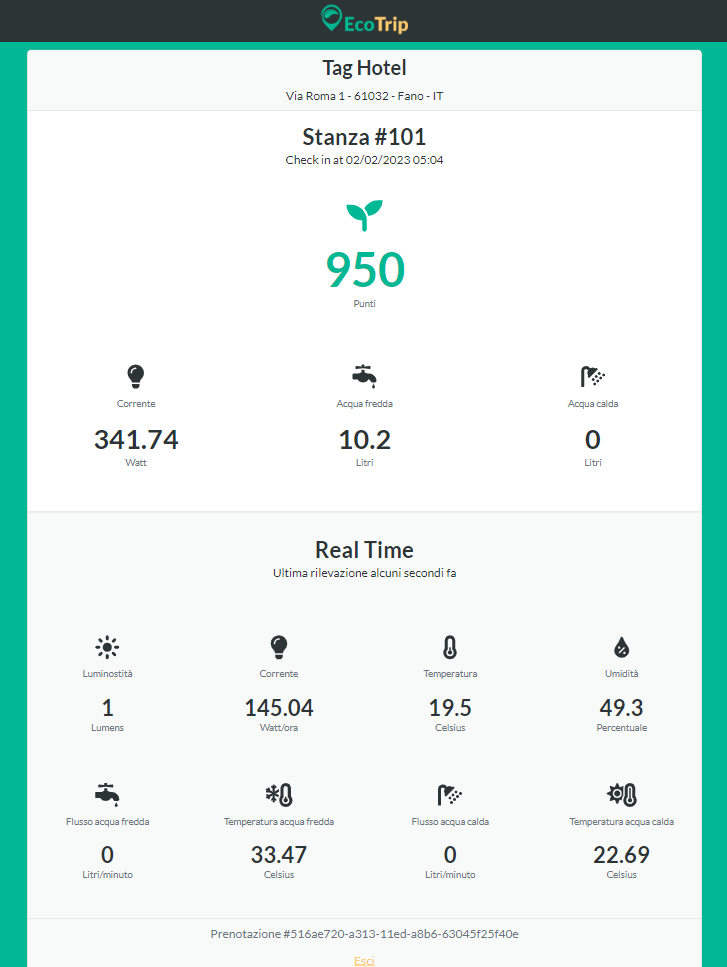
\includegraphics[width=\textwidth]{app-screen.png}
    \caption[contextmap]{Screenshot dell'app}
    \label{fig:app1}
    \end{minipage}
    \begin{minipage}{0.62\textwidth}
    \hspace*{0.5cm}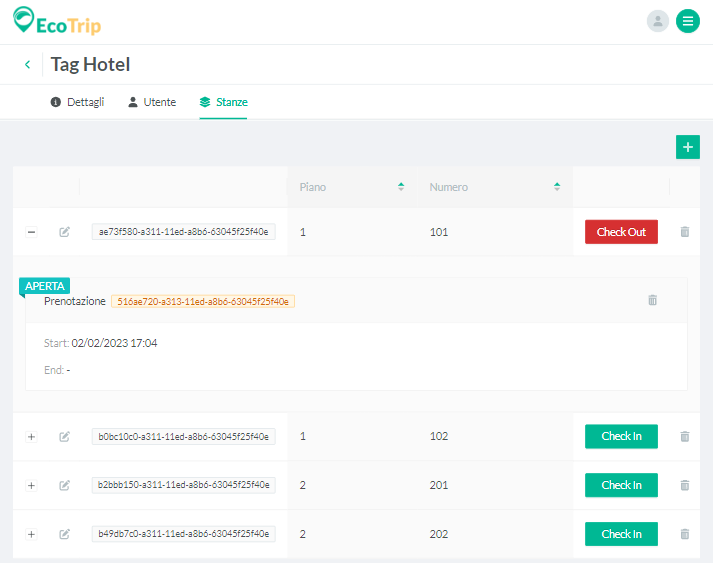
\includegraphics[width=\textwidth]{cp-screen.png}
    \caption[contextmap]{Screenshot del pannello}
    \label{fig:app2}
    \end{minipage}
    \centering
\end{figure}

\begin{figure}[H]
    \begin{minipage}{0.40\textwidth}
    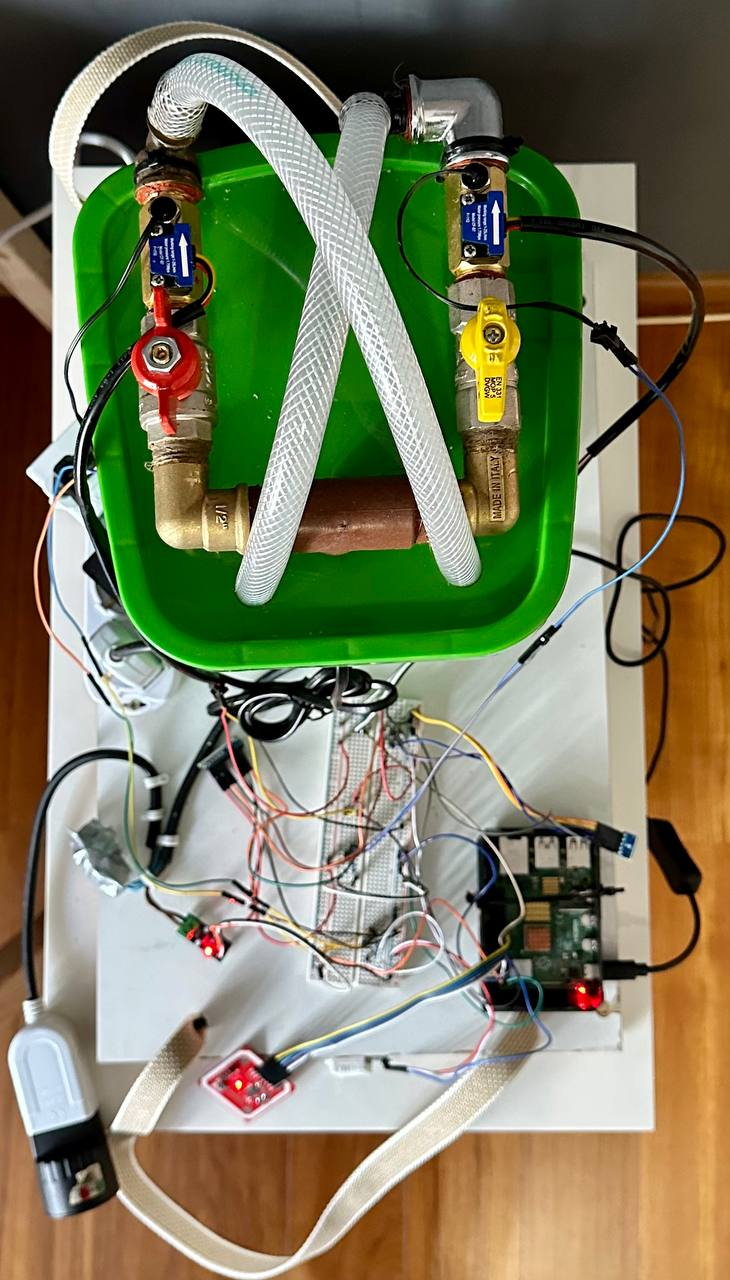
\includegraphics[width=\textwidth]{foto1.jpg}
    \label{fig:foto1}
    \end{minipage}
    \begin{minipage}{0.57\textwidth}
    \hspace*{0.5cm}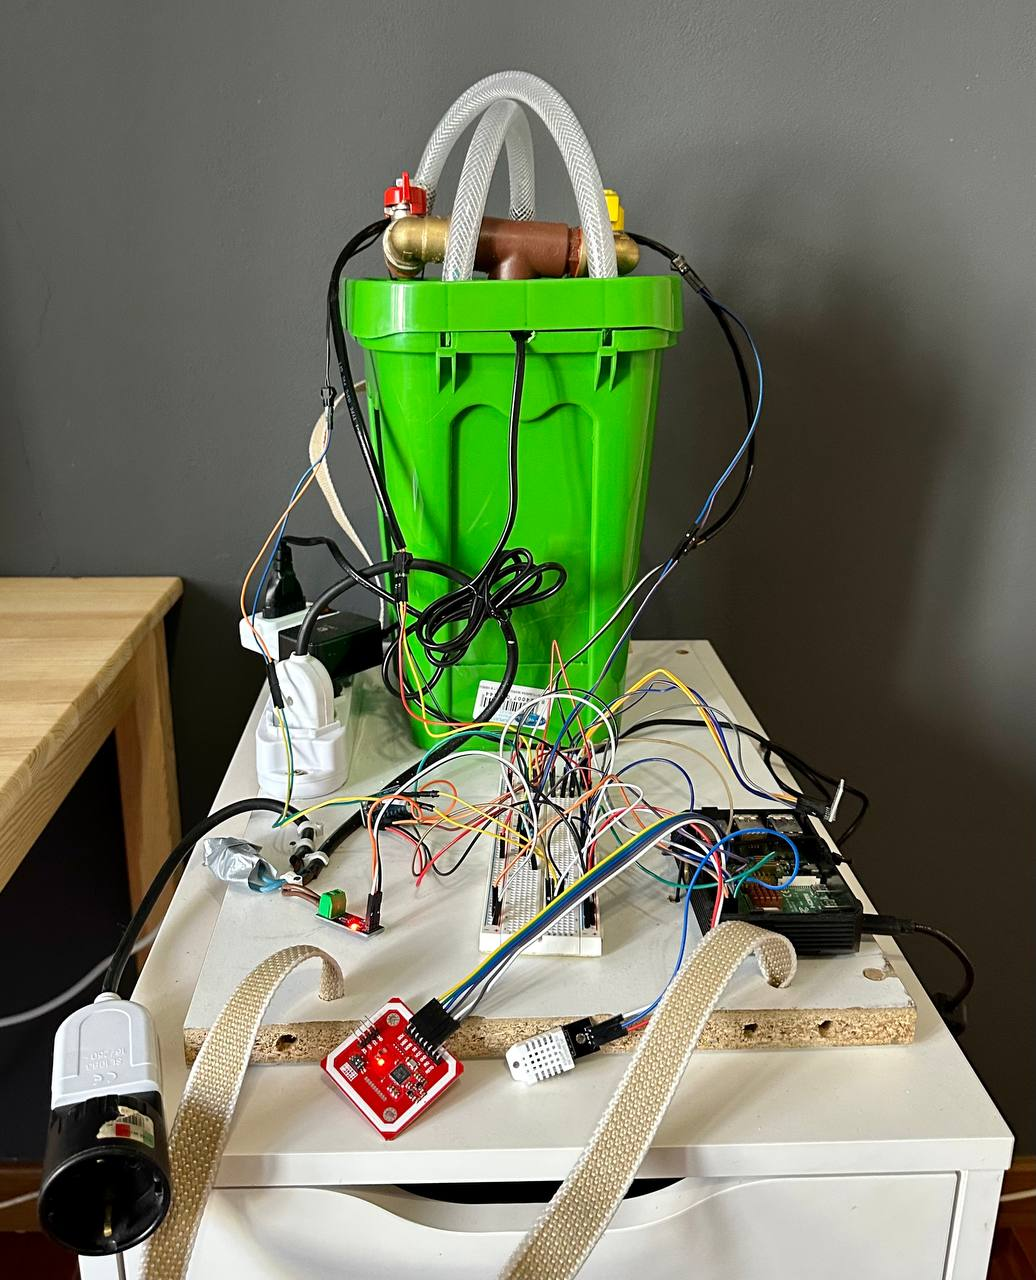
\includegraphics[width=\textwidth]{foto2.jpg}
    \label{fig:foto2}
    \end{minipage}
    \centering
    \caption[contextmap]{Foto del prototipo realizzato}
\end{figure}

%\bibliographystyle{plain}
%\bibliography{references}

\end{document}